\documentclass[titlepage,12pt]{jreport}
\usepackage{bm}
\usepackage{amsmath, amssymb}
\usepackage{type1cm}
\usepackage{ascmac}
\usepackage[dvipdfmx]{graphicx}
\usepackage{here}
\usepackage{algorithm,algorithmic} 
\usepackage{comment}
\usepackage{tabularx}
\usepackage{longtable}
\usepackage{slashbox}

\def\ex{\noindent{{\bf 例}:}}
\newcommand{\argmax}{\mathop{\rm arg~max}\limits}
\newcommand{\argmin}{\mathop{\rm arg~min}\limits}
\newcommand{\wa}{\cdot}
\newcommand{\wb}{\text{\large$cdot$}}
\renewcommand{\algorithmicrequire}{\textbf{Input:}}
\renewcommand{\algorithmicensure}{\textbf{Output:}}
\renewcommand{\bibname}{参考文献}
\newcommand{\qed}{\hbox{\rule[-2pt]{3pt}{6pt}}}
\newcolumntype{C}{>{\centering\arraybackslash}X}

%
\title{トピックモデルを考慮したタンパク質間相互作用予測}
%
\author{
東京理科大学大学院 理工学研究科 情報科学専攻\\
滝本研究室\\
6317632 宮崎 辰郎
}
%
\begin{document}
\maketitle
%

\tableofcontents
%\listoffigures


\chapter{序論\label{introduction}}
\section{背景}
タンパク質には、単体で機能するものもあれば、他のタンパク質と相互作用することで機能を果たすものもある。したがって、タンパク質の機能を解明する上でタンパク質間相互作用 ({\it Protein Protein Interaction, PPI}) は、必要不可欠なリソースである。 また、これらの相互作用に関する情報は、タンパク質間相互作用ネットワークを構築するために必要なリソースであり、生物学的プロセスの一般的な原理の理解を向上させることに役立てられている\cite{ge03}。 したがって、タンパク質間相互作用に関する研究は、生物学の分野において非常に重要な研究の一つである。 近年では、研究の重要性と計算機の発達に伴い、計算機を用いたタンパク質間相互作用に関する研究が盛んに行われている。 タンパク質間相互作用に関する研究には、タンパク質間相互作用ネットワークの可視化\cite{iragne05}\cite{STRING17}、ネットワーク分析\cite{Bader2003}、未知のタンパク質間相互作用の予測問題\cite{Lei13}\cite{Tan14}\cite{Xu10}などがあるが、本稿では、未知のタンパク質間相互作用の予測問題について取り扱う。

通常タンパク質間相互作用は、コストの高い実験によって検出され、実証されなければならない。 しかし、既知のタンパク質間相互作用およびそれらで構築されるネットワークに基づいて未知のタンパク質相互作用を予測することで、実験コストを大幅に削減することが期待できる。 

近年、機械学習やデータマイニングの領域では、ネットワークの構造で与えられるデータが増加しているため、その解析の重要性が高まり、ネットワーク構造から抽出される位相的情報やノード自身が持つ情報をリンク予測問題に活用する研究が活発に行われている。 データマイニングにおけるネットワーク解析をリンクマイニングと呼び、{\it Getoor}らは、リンクマイニングのタスクを以下のように分類している\cite{getoor05}。
\begin{itembox}[1]{リンクマイニングのタスク分類}
\begin{itemize}
	\item ノードに関連する研究
		\begin{itemize}
			\item ノードのランキング問題
			\item ノードの分類問題
			\item ノードのクラスタリング
			\item ノードの識別
		\end{itemize}
	\item リンクに関連する研究
		\begin{itemize}
			\item リンク予測問題
		\end{itemize}
	\item グラフに関連する研究
		\begin{itemize}
			\item 部分グラフの検出
			\item グラフの分類問題
			\item グラフの生成モデル
		\end{itemize}
\end{itemize}
\end{itembox}
これらのうち、本稿では、リンク予測問題を取り扱う。 リンク予測問題については、第\ref{link_prediction}節で説明する。

ノードをデータ、リンクをデータ間の関係として表現することで、様々な問題をリンク予測問題に適用することができる。 タンパク質間相互作用ネットワークでは、ノードはタンパク質、リンクはタンパク質間相互作用を表している。 したがって、既知のタンパク質間相互作用のネットワークの情報を用いて、未知のタンパク質間相互作用を予測する問題にリンク予測アルゴリズムを適用することができる。 これまでのリンク予測アルゴリズムを適用した研究では、タンパク質間相互作用ネットワークから得られる位相的情報がメインに取り扱われてきたが、近年、ノード自身が持つ情報が多く活用できるようになってきたので、位相的情報に新規情報を加え、精度向上に貢献する研究が盛んに行われている。%タンパク質間相互作用予測に関する研究では、タンパク質間相互作用ネットワークから得られる位相的情報に加え、%論文や学術誌などテキストベースのデータから自然言語処理 ({\it natural language processing}) やテキストマイニングなどの技術を用いて抽出される意味論的情報、
例えば、タンパク質の構造や、遺伝子に付与されているアノテーション情報などを用いる手法が提案されている。 これらに加え、本研究では自然言語処理などの領域で用いられるトピックモデルを考慮した新規情報を提案する。 この新規情報を、位相的情報を含む既存の特徴量に加えることで、タンパク質対の表現力を高め、リンク予測問題の精度向上をすることができることを示す。

%未知のタンパク質間相互作用を予測する研究は、分類アルゴリズムの提案、新規の特徴量の提案の2つに大別される。 分類アルゴリズムの提案は、ベイズ的手法を用いたアルゴリズム、アミノ酸配列を用いたアルゴリズム、リンク予測を用いたアルゴリズム、サポートベクタマシンやランダムフォレストなど数多くの機械学習の手法を用いたアルゴリズムなどが提案されている。 一方、新規の特徴量では、タンパク質の構造から抽出する方法、タンパク質間相互作用ネットワークから位相的情報を抽出する手法や、論文や学術誌などから自然言語処理 (natural language processing) やテキストマイニングの技術を用いて意味的情報を抽出する手法などが提案されている。

%これまでの研究では、位相的情報または意味的情報をそれぞれ単体で扱う研究がされてきた。 しかし、それぞれの情報だけでは表現力が乏しいと考える。

\section{目的}
本研究では、タンパク質間相互作用ネットワークから抽出する位相的情報や遺伝子オントロジー、アミノ酸配列から抽出されるタンパク質自身が持つ情報に加え、論文や学術誌からトピックモデルを生成することで得られる新しい特徴量を提案する。 その新規の特徴量を用いた結果、未知のタンパク質間相互作用の予測精度を向上させることができることを示す。 予測精度の向上についてはフリードマン検定及び多重比較を用いて、既存手法によって構成された特徴ベクトルとの間に、統計的に有意差があることを示す。 また、ランダムフォレストを用いて各特徴量の重要度を算出し、提案手法のタンパク質間予測における重要性について示す。

\section{貢献}
本研究の貢献は次の通りである。
\begin{itemize}
\item トピックモデルを考慮した特徴量を提案
\end{itemize}
これにより従来の情報から得られた特徴量を用いたときに比べ、タンパク質対の表現力を高め、高い精度で未知のタンパク質間相互作用を予測できることを示す。
\section{論文構成}
第\ref{ready}章では、本稿で使用する諸概念について述べる。 第\ref{proposed_method}章では既存の手法による特徴量に加え、表現力を高めることを目的とした、トピックモデルを考慮した特徴量を提案し、第\ref{valid}章では本研究で提案する特徴量の評価を行う。 第\ref{reference}章で関連研究について述べ、最後に第\ref{conclusion}章で本稿の結論を述べる。
%
\chapter{準備\label{ready}}
本章では、本稿で使用する諸概念について述べる。 まず、第\ref{protein}節でタンパク質、第\ref{PPI}節でタンパク質間相互作用について説明し、第\ref{classification}節で分類問題、第\ref{machine_learning}節で機械学習について説明する。 第\ref{link_prediction}節でリンク予測について述べる。 第\ref{hypothesis_testing}節で仮説検定について説明し、最後に第\ref{freedman_testing}節でフリードマン検定とボンフェローニ法による多重比較検定について説明する。
\section{タンパク質\label{protein}}
タンパク質は、生物の体を構成している重要な成分の一つであり、炭水化物や脂質とともに三代栄養素と呼ばれる。 20種のL-アミノ酸が50個以上結合し、鎖状に多数連結してできた高分子化合物である。 50個未満の場合は、ペプチドと呼ばれる。 人間がタンパク質を摂取したあと、体内で分解され、アミノ酸となり体内に吸収される。 
\section{タンパク質-タンパク質間相互作用\label{PPI}}
タンパク質は、単独で機能するものもあるが、その多くは他のタンパク質と作用し合うことで機能する。 この、タンパク質分子間の相互作用のことをタンパク質-タンパク質間相互作用、もしくは簡潔にタンパク質間相互作用と呼ぶ。
\section{分類問題\label{classification}}
分類問題は2値分類、マルチクラス分類、マルチラベル分類の3つに大別される。 これは用意されるクラスの数、各事例が属するクラス数によって分けられる。
\subsection{2値分類}
2値分類は、各事例があるクラスに属するか属さないかの2種類で分類するアプローチである。 また、マルチクラス分類において、クラス数が2の場合と考える事ができる。
\begin{description}
\item \ex 数字$n$を「奇数、偶数」のどちらかに分類
\end{description}
\begin{equation}
f(n) = \left\{ \begin{array}{ll}
	0 & (nが奇数)\\
	1 & (nが偶数)
	\end{array}\right.
\end{equation}
\subsection{マルチクラス分類}
マルチクラス分類は、クラス数が3以上の場合であり、各事例はどれか一つのクラスに分類される。
\begin{description}
\item \ex 学生を所属学部で分類
\begin{description}
\item クラス\\
文学部、経済学部、法学部、教育学部、理工学部
\end{description}
としたとき、学生Aを経済学部、学生Bを理工学部と複数のクラスのうちのどれか一つに分類する。
\end{description}


\subsection{マルチラベル分類}
マルチラベル分類は、マルチクラス分類と同様に、クラス数が3以上である。 マルチクラス分類では、各事例はどれか一つのクラスに分類されるが、マルチラベル分類では、各事例が複数のクラスに同時に分類されうる。
%例えば、Wikipediaは1つの記事に複数のカテゴリが付与されているので、各記事は複数のクラスに同時に分類されうる。
\begin{description}
\item \ex Wikipediaの記事を分類\\
Wikipediaの「Natural language processing」の記事は「Computational linguistics」、「Speech recognition」、「Natural language processing」の3つのクラスに同時に分類されている。
\end{description}

\section{機械学習の分類\label{machine_learning}}
機械学習は、教師あり学習 ({\it supervised learning}) と教師なし学習 ({\it unsupervised learning}) 、さらにその中間に位置する半教師あり学習 ({\it semi-supervised learning}) に大きく分けられる。
\subsection{教師あり学習}
教師あり学習とは、各入力データに対して出力(正解ラベル)が付与されている場合に行う学習の事である。 正解ラベルは、教師データとも呼ばれる。 通常入力データは、実数値ベクトルとして表現される。 このベクトルは、各入力データの特徴を表すもので、特徴ベクトルと呼ばれる。 出力は、それぞれの事例の属するクラスを表すラベルや数値が与えられる。 出力がラベルのときを分類、数値のときを回帰と呼ぶ。 例えば天気予報で晴れ、曇り、雨等を予測するとき、出力がラベルとなるので分類に相当する。

教師あり学習は、これらの入出力データを用いて、入力を出力に写像する関数や分布を求めることが目的である。
したがって、\(\bm{x}\in \bm{X}\)を入力、\(\bm{y}\in \bm{Y}\)を出力とし、\(|D|\)個の入出力ペアの集合$\bm{D}$
\begin{equation}
	\bm{D} = \{(\bm{x}^{(1)},\bm{y}^{(1)}),(\bm{x}^{(2)},\bm{y}^{(2)}),...,(\bm{x}^{(|D|)},\bm{y}^{(|D|)})\}
\end{equation}
が与えられたとき、
\begin{equation}
	f:\bm{X}\to \bm{Y}
\end{equation}
となる\(f\)や、$\bm{x}$が与えられたときの\(\bm{y}\)の条件付き確率分布である、
\begin{equation}
	p(\bm{y}|\bm{x})
\end{equation}
で表現される。 一般に\(f\)や\(p\)はパラメータを持ち、パラメータによって関数や分布が一意に決定される。 したがって、これらのパラメータを決定する問題に帰着される。 以下で、教師あり学習の代表例として、サポートベクターマシンについて述べる。
\subsubsection{サポートベクターマシン}
サポートベクターマシン({\it Support Vector Machine, SVM}) は教師あり学習を用いた線形二値分類である\cite{support}。 また、カーネル法と組み合わせて用いることで、非線形の分類も可能であるが、ここでは、線形二値分類について説明する。 教師データに与える正解ラベルはそれぞれ、正クラス ({\it positive class}) 、負クラス ({\it negative class}) と呼ばれる。 また、正クラスに属する事例は正例 ({\it positive example})、負クラスに属する事例は負例 ({\it negative example}) と呼ばれる。 事例の特徴ベクトル集合を\(\{\bm{x}^{(1)},\bm{x}^{(2)},...,\bm{x}^{(|\bm{D}|)}\}\)、事例の正解ラベルを\(\{y^{(1)},y^{(2)},...,y^{(|\bm{D}|)}\}\)とする。 このとき、正例のラベルは+1であり、負例のラベルは-1である。線形分類器の場合、分離平面の方向ベクトルを\(\bm{\omega}\)、切片を\(b\)とすると、
\begin{equation}
f(\bm{x}) = \bm{\omega} \cdot \bm{x} - b
\end{equation}
と表される。 事例\(\bm{x}\)を\(f(\bm{x}) \geq 0\)ならば正クラス、\(f(\bm{x}) < 0\)ならば負クラスに分類する。 このときのパラメータ\(\bm{\omega}\)と\(b\)を求める方法の一つにマージン最大化がある。


\begin{figure}[b]
\centering
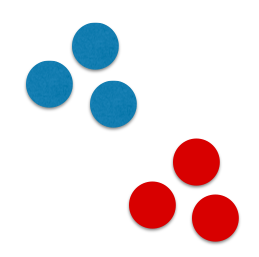
\includegraphics[width = 50mm,bb = 0 0 259 257]{img/svm1.png}

\caption{事例の分布}
\label{fig:one}
\end{figure}

例えば、図 \ref{fig:one}のように事例が分布しているとする。 ここでは2次元空間を用いて説明するが、高次元でもかまわない。 この事例を分類する平面を分離平面と呼び、最適な分離平面を構築することが目的であるが、分離平面は無数に構築することができる。 例えば図 \ref{fig:two}や図 \ref{fig:three}のように構築することができる。
\begin{figure}[htbp]
	\begin{minipage}{0.50\hsize}
		\begin{center}
			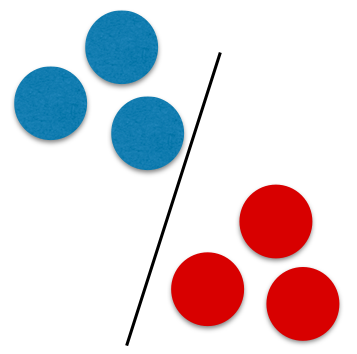
\includegraphics[width = 50mm,bb = 0 0 357 354]{img/svm2.png}
		\end{center}
		\caption{分離平面 : 例1}
		\label{fig:two}
	\end{minipage}
	\begin{minipage}{0.50\hsize}
		\begin{center}
			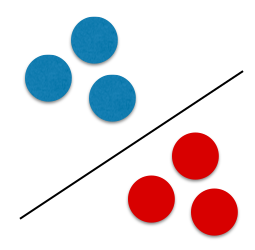
\includegraphics[width = 50mm,bb = 0 0 255 250]{img/svm3.png}
		\end{center}
		\caption{分離平面 : 例2}
		\label{fig:three}
	\end{minipage}
\end{figure}

\begin{comment}
\begin{figure}[htbp]
\centering
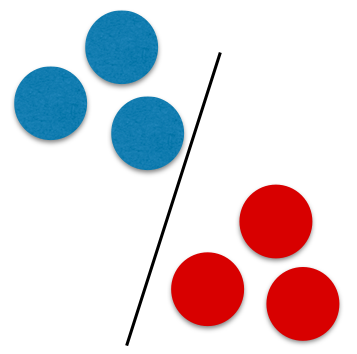
\includegraphics[width = 45mm,bb = 0 0 357 354]{img/svm2.png}

\caption{例1}
\label{fig:two}
\end{figure}
\begin{figure}[htbp]
\centering
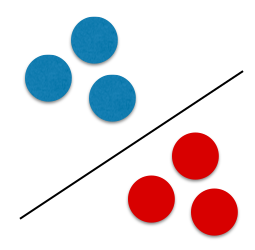
\includegraphics[width = 50mm,bb = 0 0 255 250]{img/svm3.png}
\caption{例2}
\label{fig:three}
\end{figure}
\newpage
\end{comment}
マージンとは分離面と分離面に最も近い事例を含む面との最短距離のことを言い、マージン最大化では、分離面に最も近い事例までのユークリッド距離が、最大となる分離面を決定する。 ここで、正例を1つ以上含む平面は、\(\bm{\omega} \cdot \bm{x}_{+} - b = +1\)、負例を1つ以上含む平面は、\(\bm{\omega} \cdot \bm{x}_{-} - b = -1\)で表され、これらの平面と分離平面との距離、つまりマージンは、\(\frac{1}{||\bm{\omega}||}\)となる。 また\(y^{(i)}= +1\)であるような事例については、\(\bm{\omega} \cdot \bm{x^{(i)}} - b \geq 1\)であれば良く、\(y^{(i)}= -1\)であるような事例については、\(\bm{\omega} \cdot \bm{x^{(i)}} - b \leq 1\)であれば良い。 この2つの条件は、次のようにまとめて表すことができる。
\begin{equation}
y^{(i)}(\bm{\omega} \cdot \bm{x^{(i)} - b) \geq 1}
\end{equation}
以上から、これを制約とした次の最適化問題を解けばよい。

\begin{equation}
\begin{array}{ll}
max. & \frac{1}{\bm{\omega}^{2}}\\
s.t. & y^{(i)}(\bm{\omega} \cdot \bm{x^{(i)}} - b) \geq 1 \\
	& \forall i
\end{array}
\end{equation}

また、$K$個のクラスに対して、あるクラスに入るか、他の$K-1$個のクラスのどれかに入るかの線形二値分類を解く分類器を$K$個用いることでマルチクラスに拡張する{\it One-against-rest}が提案されている。
\subsection{教師なし学習}
教師なし学習では、入力データのみが与えられ、出力の正解は与えられない。 入力データの背後に存在する規則を見い出す為に用いられ、どのような出力が望ましいかは、各学習アルゴリズムに依存する。 教師なし学習の適用対象の代表として、クラスタリングと頻出パターンマイニングの2つをあげる。
\subsubsection{クラスタリング}
入力データ群から、類似したデータをグルーピングする作業のことを、クラスタリングと呼ぶ。 また、出来上がったグループを、クラスタと呼び、単純に最も類似しているもの同士をまとめる方法を、凝集型クラスタリングと呼ぶ。

\ex はじめは、図 \ref{fig:g1}のように、すべての事例は互いに異なるクラスタに属しており、各クラスタはただ一つの事例のみを含む。 図 \ref{fig:g2}、図 \ref{fig:g3}、図 \ref{fig:g4}と進むに従って、類似しているもの同士をグルーピングしていき、少しずつ大きなクラスタが形成されていく。 また、この過程を図で表したものが図 \ref{fig:j1}の樹形図である。 クラスタリングの過程は樹形図の下から上に向かって進み、二つの線が交わっている箇所でクラスタ同士をまとめている。 交わる箇所の高さがまとめる順序を表している。 この樹形図をある高さで切ると、クラスタ集合が得られ、例えば上の方で切ると二つのクラスタが得られる。

\begin{figure}[htbp]
	\begin{minipage}{0.50\hsize}
		\begin{center}
			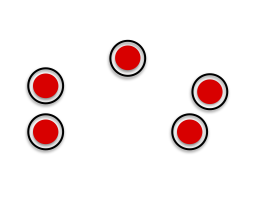
\includegraphics[width = 50mm,bb = 0 0 258 203]{img/gyou1.png}
		\end{center}
		\caption{(a)}
		\label{fig:g1}
	\end{minipage}
	\begin{minipage}{0.50\hsize}
		\begin{center}
			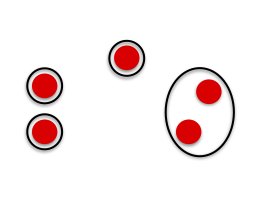
\includegraphics[width = 50mm,bb = 0 0 258 203]{img/gyou2.png}
		\end{center}
		\caption{(b)}
		\label{fig:g2}
	\end{minipage}
\end{figure}

\begin{figure}[htbp]
	\begin{minipage}{0.50\hsize}
		\begin{center}
			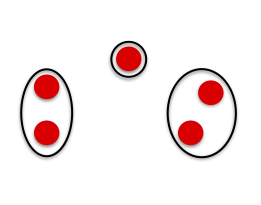
\includegraphics[width = 50mm,bb = 0 0 261 205]{img/gyou3.png}
		\end{center}
		\caption{(c)}
		\label{fig:g3}
	\end{minipage}
	\begin{minipage}{0.50\hsize}
		\begin{center}
			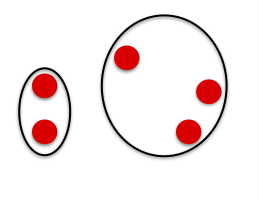
\includegraphics[width = 50mm,bb = 0 0 324 257]{img/gyou4.png}
		\end{center}
		\caption{(d)}
		\label{fig:g4}
	\end{minipage}
\end{figure}
\begin{figure}[htbp]
\centering
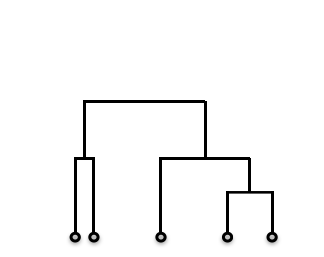
\includegraphics[width = 100mm,bb = 0 0 324 257]{img/ju1.png}
\caption{樹形図}
\label{fig:j1}
\end{figure}
\subsubsection{凝集型クラスタリング}
はじめのうちは、類似している事例同士をまとめるが、クラスタリングが進むにつれて、類似するクラスタと事例、あるいはクラスタ同士をまとめることになる。 事例同士の場合は、事例の特徴ベクトルのユークリッド距離やコサイン類似度などを測り、最も類似しているクラスタ同士を見つければ良い。 一方、クラスタ同士の場合、つまり片方あるいは両方が一つのベクトルではなく複数のベクトルからなる場合、どのように計算したら良いかは自明ではない。 そこでクラスタ同士の類似度を測るための方法として、単連結法、完全連結法、重心法の3つを紹介する。
\begin{enumerate}
\item 単連結法\\
二つのクラスタが与えられたとき、その中で最も近い事例対の類似度を、その二つのクラスタの類似度とする方法である。
\begin{equation}
sim(c_{i},c_{j}) = \max_{\bm{x_{k}}\in c_{i},\bm{x_{l}}\in c_{j}}sim(\bm{x_{k}},\bm{x_{l}})
	\label{eq:unique-sim}
\end{equation}
式 (\ref{eq:unique-sim})の値が最も大きなクラスタの対が、最も類似しているクラスタであるので、
\begin{equation}
(c_{m},c_{n}) = \argmax_{c_{i},c_{j}\in C} \max_{\bm{x_{k}}\in c_{i},\bm{x_{l}}\in c_{j}} sim(\bm{x_{k}},\bm{x_{l}})
\end{equation}
を計算すれば良い。
\item 完全連結法\\
二つのクラスタが与えられたとき、その中で類似度が最も低い事例同士の類似度を、その二つのクラスタの類似度とする方法を完全連結法と呼ぶ。
\begin{equation}
sim(c_{i},c_{j}) = \min_{\bm{x_{k}}\in c_{i},\bm{x_{l}}\in c_{j}}sim(\bm{x_{k}},\bm{x_{l}})
\end{equation}
\item 重心法 \\
各クラスタの代表ベクトルを、各クラスタが含む事例の重心ベクトルで表す。 二つのクラスタに対し、それらの代表ベクトルの類似度をこれらのクラスタ間の類似度とする方法を重心法と呼ぶ。

\begin{equation}
sim(c_{i},c_{j}) = sim(\frac{1}{|c_{i}|}\sum_{\bm{x}\in c_{i}}\bm{x},\frac{1}{|c_{j}|}\sum_{\bm{x}\in c_{j}}\bm{x})
\end{equation}
\end{enumerate}
扱っている問題によって、3つの方法を選んで使う必要がある。

凝集型クラスタリングのアルゴリズムを次に示す。 ここで、\(sim\)は、上で説明した二つのクラスタの類似度を返す関数である。
\begin{algorithm}
	\caption{凝集型クラスタリング}
	\label{algo2}
	\begin{algorithmic}[1]
		\REQUIRE 入力データ集合$D = \{\bm{x}^{(1)},\bm{x}^{(2)},...,\bm{x}^{(|D|)}\}$
	\STATE $C = \{c_{1},c_{2},...,c_{|D|}\}$
		\STATE $c_{1} = \{\bm{x}^{(1)}\},c_{2} = \{\bm{x}^{(2)}\},...,c_{|D|} = \{\bm{x}^{(|D|)}\}$\\ \# 1つのクラスタに1つの事例を割り当てる
	\WHILE {$|C| \geq 2$}
	\STATE $(c_{m},c_{n}) = \argmax_{c_{i},c_{j}\in C}sim(c_{i},c_{j})$\\ \#最も類似しているクラスタ対をみつける
	\STATE $merge(c_{m},c_{n})$\\ \#見つかったクラスタ対をまとめる
	\ENDWHILE
 \end{algorithmic}
	\label{alg:gyo}
\end{algorithm}
\subsubsection{頻出パターンマイニング}
入力データ群のうち、あるルールを満たすパターンで、出現頻度が高いパターンを列挙する手法を、頻出パターンマイニングと呼ぶ。 ルールの代表例として相関ルールがあげられる。 相関ルールとは、
\begin{equation}
X \Rightarrow Y
\end{equation}
と記述され、ある事象$X$が起こった下で、ある事象$Y$が頻繁に発生する関係を表す。 このとき、$X$を前提部、$Y$を結論部と呼ぶ。  相関ルールを抽出するアルゴリズムの一つに、{\it Apriori}\cite{Agrawal94}が広く知られている。
\subsection{半教師あり学習}
半教師あり学習は、前述の教師あり学習と、教師なし学習の中間に位置する問題である。 これは、訓練データの中に、正解が与えられないようなデータが含まれていることを指す。 入力データは大量に存在するが、正解ラベルを付与するのに膨大なコストが必要である場合に有効である。
以下に、教師なし学習の概要を示す。
\begin{itembox}[1]{教師なし学習の概要}
\begin{enumerate}
\item ラベル付きデータを用いて分類器を構築する。
\item 1で構築した分類器を用いてラベルなしデータを分類する。
\item 2で分類したラベルなしデータのうち高い確率で分類できたもののみにラベルを付与する。
\end{enumerate}
\end{itembox}
教師なし学習は、\(1\sim3\)を繰り返し行うことで学習される。

\section{リンク予測問題\label{link_prediction}}
機械学習やデータマイニングの分野では、ネットワーク構造の分析に関する研究が活発に行われている。 その一つがリンク予測である。 ネットワーク構造で表現されるデータが与えられ、その既知の位相情報から未知の位相情報を予測する問題である。 例えばソーシャルネットワークサービス (SNS) においては、与えられたネットワークの情報から、ユーザ同士の繋がりを予測する問題が例としてあげられる。 

本節では、まず、機械学習のアプローチをリンク予測問題で扱えることを述べ、次に、機械学習を用いてリンク予測を行うときに、用いるネットワーク構造から得られる位相的情報について説明する。 最後に、それを特徴量とし2値分類に適応することを説明する。

\subsection{機械学習アプローチを用いたリンク予測}
各リンクが存在するか否かを予測すれば良いので、入力をノード対の情報、出力を各ノード対におけるリンクの有無とする2値分類問題として考えることができる。 すなわち、各ノード対の特徴ベクトルを抽出し、機械学習アプローチを適用すれば良い。 したがって、各ノード対の特徴ベクトルを定義することが、機械学習アプローチを用いたリンク予測問題において重要なステップとなる。 各ノード対に用いることのできる情報は、ネットワークの位相的情報と、ノード自身が持つ情報の2つに大別される。
\begin{itemize}
	\item ネットワークの位相的情報 \par ノードの隣接、またはその周辺ノードのリンク構造から得られる情報である。 共通の知人を持つ人同士は、その人同士も知人である可能性が高いといった具合である。
	\item ノード自身が持つ情報 \par \ex ソーシャルネットワークサービスにおけるユーザのIDや年齢、趣味など タンパク質間相互作用ネットワークにおけるタンパク質の発言情報や配列情報など
\end{itemize}

各リンクの有無を、2値分類問題として扱うことで、機械学習のアプローチを、リンク予測に適用することが可能である。 %一般的に、各ノード間におけるリンクの有無を扱う2値分類問題として考えることができる。
通常の機械学習アルゴリズムが、各ノードに対する特徴ベクトルを定義し、その特徴ベクトルを基にノードの性質などを予測しているのに対し、機械学習アプローチを用いたリンク予測では、各ノード対に対する特徴ベクトルを定義し、その特徴ベクトルを基に、ノード対の性質 (リンクの有無など) を予測している。

したがって、各ノード対を表す特徴ベクトルを定義することで、通常の機械学習アプローチをリンク予測に適用することが可能である。

\subsection{ネットワーク構造から得られる情報\label{topology-info}}
リンク予測におけるネットワークとは、各データをノードとし、データ間の関係をリンクとして表現したものである。 ここでは、ネットワークに存在する任意の2つのノードの周辺ノードの情報を用いて定義される7つのノード間の類似尺度の定義を示す。

以下、$i$番目のノードを$x_i$とし、$x_i$に隣接するノードの集合を$\Gamma(x_i)$とする。
\begin{enumerate}
	\item {\it common neighbors}
\begin{eqnarray}
	S^{CN}(x_{i}, x_{j}) \equiv |\Gamma(x_{i}) \cap \Gamma(x_{j})| 
\end{eqnarray}
{\it common neighbors}はリンク予測で最も使われる指標の一つである。 {\it common neighbors}は$x_{i}$と$x_{j}$が共通の隣接ノードを多く持っているほど、$x_{i}$と$x_{j}$間にはリンクが現れやすいことを表現している。 ソーシャルネットワークを例に挙げると、「共通の知人が多い2人は、互いに知人である可能性が高い」という具合である。

\item {\it Jaccard's coefficient}
\begin{eqnarray}
	S^{JC}(x_{i}, x_{j}) \equiv \frac{|\Gamma(x_{i}) \cap \Gamma(x_{j})|}{|\Gamma(x_{i}) \cup \Gamma(x_{j})|}
\end{eqnarray}

{\it Jaccard's coefficient}は{\it common neighbors}を正規化した式で得られる。すなわち、2つの隣接ノード集合の和集合に対する共通の隣接ノード集合の割合を表現している。

\item {\it Adamic/Adar index}
\begin{eqnarray}
	S^{AAI}(x_{i}, x_{j}) \equiv \sum_{z \in \Gamma(x_{i}) \cap \Gamma(x_{j})} \frac{1}{\log{|\Gamma(z)|}}
\end{eqnarray}

{\it Adamic/Adar index}は、{\it Adamic}らが提案した、2つのウェブページ間における初めての類似性尺度であり、{\it common neighbors}の重み付き和で表現され、隣接するノードが持つ隣接ノード数に応じて、重みが割り当てられる\cite{adamic03}。 隣接ノードの少ないノードを共通して隣接ノードとして持つ場合、重みは大きくなり、隣接ノードの多いノードを共通して隣接ノードとして持つ場合、重みは小さくなる。 ソーシャルネットワークを例に挙げると、「知人の少ない人の知人である二人は、その人同士も知人である可能性が高く、知人の多い人を共通の知人に持っていても、その人同士が知人であるかどうかを知るための情報には、不十分である」という具合である。

\item {\it Preferential attachment}
\begin{eqnarray}
	S^{PA}(x_{i}, x_{j}) \equiv |\Gamma(x_{i}) \times \Gamma(x_{j})|
\end{eqnarray}

{\it Preferential attachnent}は、「隣接ノードが多いノードほど、新たにリンクが張られやすい」ことを仮定している\cite{pa02}。 定義を見てわかる通り、{\it Preferential attachment}はそれぞれのノードの隣接するノードの集合の直積集合の要素数で与えられるが、結果として、2つのノードが持つ隣接ノード数の掛け算と同値である。 したがって、共通の隣接ノードを持っている必要はない。

\item {\it Resource allocation}
\begin{eqnarray}
	S^{RAI}(x_{i}, x_{j}) \equiv \sum_{z \in \Gamma(x_{i}) \cap \Gamma(x_{j})} \frac{1}{|\Gamma(z)|}
\end{eqnarray}

{\it Resource allocation}は{\it Adamic/Adar index}に似ているが、{\it Adamic/Adar index}が重みを割り当てるときに対数の逆数を用いていたのに対し、{\it Resource allocation}は、隣接ノード集合の要素数の逆数で定義される。 これは、{\it Adamic/Adar index}より、隣接するノード数が多いノードを共通の隣接するノードに持つ場合に、大きくペナルティを課していることを表している。

\item {\it Sorensen Dice coefficient}
\begin{eqnarray}
	S^{DSC}(x_{i}, x_{j}) \equiv \frac{2|\Gamma(x_{i}) \cap \Gamma(x_{j})|}{|\Gamma(x_{i})| + |\Gamma(x_{j})|}
\end{eqnarray}

{\it Jaccard's coefficient}では、2つの隣接ノード集合の和集合を用いて{\it common neighbors}を正規化している。 しかし、2つの隣接ノード集合の差集合の要素数が多いと、{\it Jaccard's coefficient}は、小さく見積もられてしまう。 {\it Sorensen Dice coefficient}は、この欠点を緩和するために、隣接ノード集合の積集合に重きをおき、差集合の要素数の影響を抑えることを目的として提案された。 

\item {\it Overlap coefficient}
\begin{eqnarray}
	S^{overlap}(x_{i}, x_{j}) \equiv \frac{|\Gamma(x_{i}) \cap \Gamma(x_{j})|}{min \{ |\Gamma(x_{i})| , |\Gamma(x_{j})| \} }
\end{eqnarray}

{\it Jaccard's coefficient}の欠点である、隣接ノード集合の差集合の影響を緩和するために、{\it Sorensen Dice coefficient}が提案されたが、それでもなお、差集合の要素数が膨大になった場合に、小さく見積もられてしまう。 {\it Overlap coefficient}では、差集合の要素数の影響を極限まで抑えることを目的として提案された。 {\it Jaccard's coefficient}や{\it Sorensen Dice coefficient}に比べ、隣接ノード集合の積集合の要素数に重きをおいた類似性尺度と言える。
\end{enumerate}

\subsection{ノード対に関する特徴量を用いた2値分類}
ノード対$(x_i, x_j)$に対する特徴量を、位相構造から得られる情報やノード自身が持つ情報などを組み合わせ、$\bm{v}^{(i, j)} = [v^{(i, j)}_1, v^{(i, j)}_2, \cdots, v^{(i, j)}_n]$と表せたする。 ここで、$\bm{v}^{(i, j)}_k$をノード$x_i$と$x_j$における$k$番目の位相的情報であり、$n$は位相的情報の総数である。 例えば、上で説明した7つの位相的情報を用いるとき、$\bm{v}^{(i, j)} = [S^{CN}(x_i, x_j), S^{JC}(x_i, x_j), \cdots, S^{overlap}(x_i, x_j)]$、$n = 7$となる。またこのノード対にリンクが存在することが既知であれば、ラベルを$y^{(i,j)} = 1$、リンクが存在しないことが既知であれば、$0$とする。 これらの既知のノード対の情報を教師データとして与え、通常の機械学習アプローチ (ランダムフォレストや、サポートベクターマシンなど) を適用することで、未知のノード対のリンクに関する知見を予測することができる。

\section{仮説検定\label{hypothesis_testing}}
本節では、まず第\ref{sub:hypothesis_testing}項で仮説検定の考え方について述べ、そのあと第\ref{null-hypothesis}項で帰無仮説と対立仮説について述べ、最後に、第\ref{rejection-region}項で両側検定と片側検定検定について説明をする。
\subsection{仮説検定の考え方\label{sub:hypothesis_testing}}
仮説検定とは、統計的仮説の有意性に関する検定である。 つまり、仮説のもとで期待されるものと、実際に観測された結果との間の違いが、偶然生じたものか否かを確率の基準で評価する。 例えば、1865年にメンデルが行った、エンドウ豆の色や形状に関する遺伝形質を調査した実験で得られた実験データが、理論上の仮説に合致しているかどうかの検証があげられる。 この実験結果 (表 \ref{tab:mendel}) から、メンデルは各型の度数の比が9:3:3:1になると考えた。 しかし、厳密には9:3:3:1になっていないことは自明である。 ここで重要なことは、理論比からのずれが誤差の範囲内なのかどうかという点である。 理論比からのずれが誤差の範囲内ではない場合、統計学では、仮説は有意であるという。 ここで有意であるとは偶然起こったとは判断しかねることを意味する。
\begin{table}[tbp]
	\begin{center}
		\caption{メンデルが行ったエンドウ豆についての実験データ}
		\begin{tabular}{c|ccccc} \hline
			型 & 黄 $\cdot$ 丸 & 黄 $\cdot$ しわ & 緑 $\cdot$ 丸 & 緑 $\cdot$ しわ & 計 \\ \hline
			観測度数 & 315 & 101 & 108 & 32 & 556 \\ \hline
			理論比 & 9 & 3 & 3 & 1 & (16)\\ \hline 
		\end{tabular}
		\label{tab:mendel}
	\end{center}
\end{table}

もう一つ、コイン投げの例をあげて説明する。 例えば、コインを10回投げたときに8回表が出た場合、このコインに歪みがないと言えるかどうかという問題があげられる。 「歪みがない」という仮説のもとでは、$p = 1 / 2$、$N = 10$であるため、$Bi(10, 1/2)$の二項分布に従う。 もし仮説が正しい場合、表の回数を確率変数$X$で表すと、二項分布の計算から、$P(X \geq 8) = 0.0537$であるから、$X = 8$は、「歪みがない」という仮説のもとでは、コインが8回 (以上)出る確率は、約5\%である。 このことから、観測されるはずのない値であると主張することができる。 したがって、「歪みがない」という仮説が間違っているという結論を下す。 このことを、仮説を棄却 ({\it reject}) すると表現する。 しかし、約5\%でも確率が0ではないので、起こりうる確率であると主張することもできる。 そこで、仮説を棄却するときの基準、つまり、仮説が有意である確率の基準を定める必要がある。 この基準を有意水準 ({\it significance level}) といい$\alpha$で表す。 有意水準$\alpha$を下回れば、起こり得ない確率とする。 今回のコインの例では、有意水準を$\alpha = 0.1$にした場合、$0.0537$は、有意水準を下回るので、仮説は棄却される。 しかし、有意水準を$\alpha = 0.01$にした場合、有意水準を上回るので、帰無仮説は棄却されない。

%、あるいは有意水準$\alpha$で有意であると表現する。 


\subsection{帰無仮説と対立仮説\label{null-hypothesis}}
第\ref{sub:hypothesis_testing}項では仮説検定の考え方について述べた。 例に挙げたコインを10回投げる試行において、コインに歪みがないという仮説は、有意水準$\alpha = 0.1$で棄却された。 このときにたてた仮説を、帰無仮説 ({\it null hypothesis})とよび、$H_{0}$で表す。 帰無仮説$H_{0}$のもとで計算された確率が有意水準を下回る場合には、帰無仮説$H_{0}$は正しくないと考える。

帰無仮説$H_{0}$が棄却されたときに採用する仮説を明示的に考えることがある。 それを対立仮説 ({\it alternative hypothesis}) とよび、$H_{1}$で表す。 

仮説検定の結果で積極的に主張できることは、帰無仮説$H_{0}$を棄却し対立仮説$H_{0}$が正しいと判断できるときだけである。 したがって、実験者が主張したいことを対立仮説にしておけば良い。 コインの例では、コインに歪みがあることを対立仮説とすれば良い。

まとめると、仮説検定とは、標本によって得られた情報を用いて、母集団に関する主張を採択するか棄却するかを判断することである。 $H_{0}$のもと標本$X = x$が偶然生じたものなのか否かを、裾の確率を用いて測定し、その確率が有意水準$\alpha$を下回れば帰無仮説を棄却し、そうでない場合は帰無仮説を採択 ({\it accept}) する。

%二項分布の計算結果である、$0.0537$を観測されるはずのない偶然、つまり有意であると考えたが、一般に、有意である確率の基準を定める必要がある。 この基準を有意水準 ({\it significance level}) といい$\alpha$で表す。 先ほどの例だと、$\alpha = 0.1$と定義した場合は$0.0537$は有意であると判断できるが、$\alpha = 0.01$とした場合は、$0.0537$は十分に起こりうる確率であるので、$X = 14$は有意であるとは言えず、仮説は棄却されない。

$p$値とは「帰無仮説$H_0$が正しいという仮定の下で、偏った統計検定量が得られる確率」を表している。 コインの例で$P(X \geq 8)$の確率を求めたが、この値が$p$値である。 したがって、有意水準を$p$値が下回ったときに帰無仮説を棄却し、有意差があったと結論づけることができる。


\subsection{両側検定と片側検定\label{rejection-region}}
帰無仮説は差がない状態を表すのに対し、対立仮説は差がある状態を表す。 差の有無を考える場合と大小関係を考慮する場合に応じて、両側対立仮説と片側対立仮説がある。 両側対立仮説に対する検定を両側検定 ({\it two-sided test})、片側対立仮説に対する検定を片側検定 ({\it one-sided test}) と呼ぶ。

コインの例では、コインに歪みがあることを主張したいので、帰無仮説$H_{0}: p = 1 / 2$、対立仮説$H_{1} : p \neq 1 / 2$とたてて仮説検定を行う。 これは両側対立仮説の例であり、それに対応する検定は両側検定である。

一方、試験勉強に効果があることを主張したいとする。 つまり、帰無仮説を$H_{0} : $ 「試験勉強をする前とした後で試験の結果に差がない」とする。 このことを表現するため、試験の結果の変化量の母平均$\mu$に関して$H_{0} : \mu = 0$とすれば良い。 試験勉強に効果がある場合、$\mu$は大きくなるので、対立仮説には$H_{1} : \mu > 0$を想定すれば良い。 これは、片側対立仮説の例であり、それに対応する検定は片側検定である。

標本から得られた統計量の値がある領域の値をとるときに、帰無仮説を棄却するのが一般的な手順であり、帰無仮説を棄却する範囲を棄却域 ({\it rejection region})とよび、採択する領域を採択域 ({\it acceptance region}) とよぶ。


\section{フリードマン検定とボンフェローニ法による多重比較検定\label{freedman_testing}}
本節では、第\ref{sub:friedman}項で、3群以上の対応のあるデータに対する差の検定であるフリードマン検定について説明し、第\ref{sub:tajuu}項でボンフェローニ法による多重比較検定について説明する。
\subsection{フリードマン検定\label{sub:friedman}}
フリードマン検定とは、3群以上の対応のあるデータについて、ノンパラメトリックで代表値の差の検定である。 帰無仮説$H_{0}$を「各処理対の母代表値に差はない」、対立仮説$H_{1}$を「各処理対の母代表値に差がある」とし、有意水準$\alpha$で両側検定を行う。

ここでは4種類の肥料間で収穫量に差があるかを検定することを例に挙げて説明する。 例で扱うデータは表 \ref{tab:friedman}を参照されたい。

\begin{table}[btp]
	\begin{center}
		\caption{4種類の肥料による収穫量}
		\begin{tabular}{|c||c|c|c|c|} \hline
			品種 & 肥料1 & 肥料2 & 肥料3 & 肥料4  \\ \hline \hline
			品種1 & 10 & 20 & 14 & 18 \\ \hline
			品種2 & 5 & 30 & 14 & 9 \\ \hline
			品種3 & 4 & 20 & 10 & 11 \\ \hline 
		\end{tabular}
		\label{tab:friedman}
	\end{center}
\end{table}

まずはじめに帰無仮説と対立仮説を次のようにたてる。
\begin{itemize}
	\item 帰無仮説$H_{0}$ : 収穫量に差はない。
	\item 対立仮説$H_{1}$ : 収穫量に差がある。
\end{itemize}

次に、各肥料ごとに収穫量$x_{ij}$の小さい順に順位$R_{ij}$をつける。 ただし、$x_{ij}$は$j$番目の肥料を用いた場合の$i$番目の品種の収穫量を表し、$R_{ij}$は$x_{ij}$の順位を表す。 同順位が存在する場合は、平均順位をそれぞれにつける。 一般に、対照群(例の場合、品種) の数を$n$、処理群(例の場合、肥料)の数を$m$とすると、$1 \leq i \leq n$、$1 \leq j \leq m$であり、$1 \leq R_{ij} \leq m$となる。 

順位をつけ終えたら、各処理ごとに順位の和と順位の2乗和を計算する。
\begin{eqnarray}
	R_{\wa j} &=& \sum_{i = 1}^{n}R_{ij} \\
	R^{2}_{\wa j} &=& \sum_{i = 1}^{n}R^{2}_{ij}
\end{eqnarray}
表 \ref{tab:friedman}を下に、各処理ごとの順位の和と順位の2乗和を計算した結果が表 \ref{tab:friedman_junni}である。
\begin{table}[tbp]
	\begin{center}
		\caption{4種類の肥料に収穫量の順位}
		\begin{tabular}{|c||c|c|c|c|} \hline
			品種 & 肥料1 & 肥料2 & 肥料3 & 肥料4  \\ \hline \hline
			品種1 & 1 & 4 & 2 & 3 \\ \hline
			品種2 & 1 & 4 & 3 & 2 \\ \hline
			品種3 & 1 & 4 & 2 & 3 \\ \hline 
			$R_{\wa j}$ & 3 & 12 & 7 & 8\\ \hline
			$R^{2}_{\wa j}$ & 9 & 144 & 49 & 64\\ \hline
		\end{tabular}
		\label{tab:friedman_junni}
	\end{center}
\end{table}

次に、以下で定義された検定統計量を計算する。 検定統計量$\chi^{2}(m - 1)$は自由度$m - 1$の$\chi^{2}$分布に従う。

\begin{eqnarray}
	\chi^{2}(m - 1) = \frac{12}{nm(m + 1)}\sum_{j = 1}^{m}R^{2}_{\wa j} - 3n(m + 1)
\end{eqnarray}

肥料と収穫量の例では、$\chi^{2}(m - 1) = 8.2$であり自由度3の$\chi^{2}$分布に従う。

有意水準$\alpha$で検定を行う場合、$\chi^{2}(m - 1) > \chi^{2}(m - 1)_{\alpha}$ならば帰無仮説$H_{0}$は有意水準$\alpha$で棄却され、$\chi^{2}(m - 1) \leq \chi^{2}(m - 1)_{\alpha}$ならば帰無仮説$H_{0}$は棄却されない。 例の場合、自由度3の$\chi^{2}$分布において、$\chi^{2}(4 - 1)_{0.05} = 7.81$なので、帰無仮説は棄却され、「肥料間に差がある」という結果を得る。

\subsection{ボンフェローニ法による多重比較検定\label{sub:tajuu}}
\subsubsection{多重比較検定が必要な理由}
	多重比較とは、3群以上の観測値において、どの群間に有意差があるのかを検定する方法である。 パラメトリック法では、母平均の差を、ノンパラメトリック法では、平均順位の差を比較する。 どの群間に有意差があるのかを検定するために、群の各対で繰り返し検定を行う場合、多重性によって、定めた有意水準に比べて第1種の誤りの確率が大きくなってしまう。 例えば、A、B、Cの3群があったとして、各対(A, B)、(A, C)、(B, C)の差の検定で帰無仮説が採択される確率をそれぞれ$P_{AB}$、$P_{AC}$、$P_{BC}$、棄却される確率を$P_{AB^{c}}$、$P_{AC^{c}}$、$P_{BC^{c}}$、有意水準を$\alpha$としたとき、

\begin{eqnarray}
	P_{AB} = P_{AC} = P_{BC} = 1 - \alpha \\
	P_{AB^{c}} = P_{AC^{c}} = P_{BC^{c}} = \alpha \nonumber \\
\end{eqnarray}
となる。 第1種の誤りは、少なくとも一つの検定で帰無仮説が棄却されたときなので、その確率を$P_{er}$としたとき、

\begin{eqnarray}
	P_{er} = 1 - P_{AB} \cdot P_{AC} \cdot P_{BC} = 1 - (1 - \alpha)^{3}
\end{eqnarray}
となる。 例えば、有意水準$\alpha = 0.05$で検定を行うとき、$P_{er} = 1 - (1 - 0.05)^{3} = 0.142625$となるので、通常の第1種の誤りの確率の約3倍となってしまう。 これが、群の各対で検定を繰り返し行うことのできない理由である。

\subsubsection{ボンフェローニ法}
多重比較は、第1種の誤りの確率が大きくなることを防ぐ。 統計量を用いた方法や$p$値を調整する方法があるが、ボンフェローニ法は$p$値を調整する方法である。

具体的には、検定数 (検定する対の数)が$N$のとき、それぞれの検定の有意水準$\alpha$を$\alpha/N$に変更する方法である。 例えば、10対で検定を行う場合、全ての検定において$\alpha/10$を有意水準として使う。

\begin{comment}
	
本節では、前節で用いた肥料と収穫量の関係を例に挙げて多重比較について説明する。

まず、帰無仮説と対立仮説を以下のように立てる。
\begin{itemize}
	\item 帰無仮説 $H_{0}$ : 各肥料間の収穫量に差はない。
	\item 対立仮説 $H_{1}$ : 各肥料間の収穫量に差がある。
\end{itemize}

次に、フリードマン検定のときと同様に各処理ごとに順位をつける。 順位をつけ終えたら、各処理ごとに平均順位 $\overline{R}_{\wa j}$と分散を次の定義にしたがって計算する。
\begin{eqnarray}
	\overline{R}_{\wa j} &=& \frac{R_{\wa j}}{n} \\
	V &=& \sum_{i = 1}^{n}\sum_{j = 1}^{m}(R_{ij} - \frac{m + 1}{2})^{2}
\end{eqnarray}
表 \ref{tab:friedman}を下に順位、順位の平均を計算した結果が表 \ref{tab:friedman_junni_of_mean}である。 また分散は$V = 15.0$である。

\begin{table}[htb]
	\begin{center}
		\caption{4種類の肥料に収穫量の平均順位}
		\begin{tabular}{|c||c|c|c|c|} \hline
			品種 & 肥料1 & 肥料2 & 肥料3 & 肥料4  \\ \hline \hline
			品種1 & 1 & 4 & 2 & 3 \\ \hline
			品種2 & 1 & 4 & 3 & 2 \\ \hline
			品種3 & 1 & 4 & 2 & 3 \\ \hline 
			$\overline{R}_{\wa j}$ & 1.00 & 4.00 & 2.33 & 2.67\\ \hline
		\end{tabular}
		\label{tab:friedman_junni_of_mean}
	\end{center}
\end{table}

処理$_{i}$と処理$_{j}$の対比較のための検定統計量$S_{ij}$は次式で定義される。 また、$S_{ij}$は自由度$m - 1$の$\chi^{2}$分布に従う。
\begin{eqnarray}
	S_{ij} = \frac{n^{2}(m - 1)(\overline{R}_{\wa i} - \overline{R}_{\wa j})^{2}}{2V}
\end{eqnarray}

表 \ref{tab:friedman_junni_of_mean}を下に、各処理対の検定統計量を計算した結果、表 \ref{tab:test_static}を得る。

\begin{table}[htb]
	\begin{center}
		\caption{各処理対の検定統計量}
		\begin{tabular}{|c|c|c|} \hline
			処理対 & 検定統計量 & 結果 \\ \hline
			肥料1 vs 肥料2 & 8.10 & ** \\ \hline
			肥料1 vs 肥料3 & 1.59 & n.s. \\ \hline
			肥料1 vs 肥料4 & 2.51 & n.s.\\ \hline
			肥料2 vs 肥料3 & 2.51 & n.s.\\ \hline
			肥料2 vs 肥料4 & 1.59 & n.s.\\ \hline
			肥料3 vs 肥料4 & 0.10 & n.s.\\ \hline
		\end{tabular}
		\\ * : 有意($p < 0.05$), n.s. : 非有意
		\label{tab:test_static}
	\end{center}
\end{table}

表 \ref{tab:test_static}に示した検定統計量は全て自由度3の$\chi^{2}$分布に従うので、 有意水準$\alpha=0.05$で検定を行う場合、$\chi^{2}(3) > \chi^{2}_{0.05}(3)$ならば帰無仮説$H_{0}$は有意水準$\alpha$で棄却され、$\chi^{2}(3) \leq \chi^{2}_{0.05}(3)$ならば帰無仮説$H_{0}$は棄却されない。 今回自由度$3$の$\chi^{2}$分布において、$\chi^{2}_{0.05}(3) = 7.81$なので、肥料1と肥料2の間に差があるといえ、その他の肥料間に差があるとはいえないという結論を得られる。
\end{comment}



\chapter{提案手法\label{proposed_method}}
本章では、第\ref{LDA}節で文書中の単語のトピックを確率的に求める言語モデルである{\it LDA}について説明し、そのあとに、第\ref{sec:proposed-method}節で、提案手法である、トピックモデルを考慮したタンパク質対に関する情報について述べる。
\section{Latent Diriclet Allocation(LDA)\label{LDA}}
文書中の単語の潜在トピックを確率的に推論するモデルを{\it LDA}と呼ぶ\cite{lda03}。 {\it LDA}は、各単語は潜在的なトピックを持ち、同じトピックを持つ単語は同じ文書に出現しやすいことを仮定している。 その潜在的なトピックの分布の事前分布にディリクレ分布を仮定して生成する。 以下にディリクレ分布、多項分布の定義、{\it LDA}の生成過程、{\it LDA}のグラフィカルモデルを記す。
\begin{description}
\item [ディリクレ分布(Dirichlet distribution)]
\end{description}
\begin{equation}
Dir(\bm{\theta} | \bm{\alpha}) = \frac{\Gamma(\sum_{i=1}^{k}\alpha_{i})}{\prod_{i=1}^{k}\Gamma(\alpha_{i})}\prod_{i=1}^{k}\theta_{i}^{\alpha_{i}-1} \propto \prod_{i=1}^{k}\theta_{i}^{\alpha_{i}-1}
\end{equation}
\begin{description}
\item [多項分布(Multinomial distribution)]
\end{description}
\begin{equation}
Multi(\bm{n}|\bm{\theta}) = \frac{\Gamma((\sum_{k=1}^{K}N_{k}) + 1)}{\prod_{k=1}^{K}\Gamma(N_{k}+1)}\prod_{k=1}^{K}\theta_{k}^{N_{k}}
\end{equation}
\begin{itembox}[1]{LDAの生成過程}
\bf{トピックの確率分布を選択}$\bm{\theta_{m}} \sim Dir(\bm{\theta}_{m}|\bm{\alpha}) \;\;\;(m = 1,...,M)$\\
\bf{トピック毎に単語出現確率分布を生成}$\bm{\phi_{k}} \sim Dir(\bm{\phi}_{k}|\bm{\beta}) \;\;\;(k = 1,...,K)$\\
\bf{単語の潜在トピックを生成}$z_{m,n} \sim Multi(z_{m,n}|\bm{\theta_{m}}) \;\;\; (n = 1,...,N_{m})$\\
\bf{トピックに応じた確率で単語を生成}$w_{m,n} \sim Multi(w_{m,n}|\bm{\theta_{z_{m,n}}})\;\;\;(n = 1,...,N_{m})$
\end{itembox}
\begin{figure}[htbp]
\centering
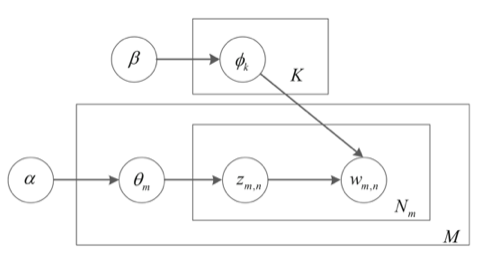
\includegraphics[height = 85mm ,width = 130mm]{img/lda.png}
	\caption{{\it LDA}のグラフィカルモデル}
\label{fig:l1}
\end{figure}

グラフィカルモデルにおける各変数の意味は次のようになる。
\begin{screen}
\begin{itemize}
\item M:文書数
\item $N_{m}$:文書mに含まれる単語数
\item k:トピック数
\item $w_{m,n}$:文書m、単語nの語彙インデックス
\item $z_{m,n}\in [i...,k]$:文書mにおける単語nのトピック番号
\item $\bm{\theta_{m}}$ 文書mに置けるトピックの出現確率
\item $\bm{\phi_{k}}$:トピックkにおける語彙の出現確率
\item $\bm{\alpha}$:トピックの出現確率の偏りを表すパラメータ
\item $\bm{\beta}$:語彙の出現確率の偏りを表すパラメータ
\end{itemize}
\end{screen}
図 \ref{fig:l1}から、$\theta \rightarrow z \rightarrow w$の順で生成されることが分かる。 また、$\theta$は$M$回、$z$は$N$回生成される。 単語分布$p(w|z)$、トピック$p(z|\theta)$、トピック分布$p(\theta|\alpha)$を用いると、
\begin{equation}
p(w,z,\theta) = p(w|z)p(z|\theta)p(\theta|\alpha)
\end{equation}
と表される。 したがって、文書$\bm{w}_{m} = {w_{m,1},...,w_{m,n}}$、文書全体$\bm{w}$について、
\begin{equation}
p(\bm{w}_{m},z,\theta) = p(\theta|\alpha)\prod_{n}p(w_{m,n}|z_{m,n})p(z_{m,n}|\theta)
\label{equation:topicmodel}
\end{equation}
\begin{equation}
\begin{split}
p(\bm{w}) = 
&\int \sum_{z}p(\bm{w},z,\theta) d\theta\\
=&\frac{\Gamma(\sum_{k}\alpha_{k})}{\prod_{k}\Gamma(\alpha_{k})}\int (\prod_{k}\theta_{k}^{\alpha_{k}-1})\prod_{n}\sum_{k}p(w_{n}|k)\theta_{k}d\theta
\end{split}
\label{equation:lda}
\end{equation}
と計算できる。 式 (\ref{equation:lda})の積分は変分ベイズ法等を用いて推定する。

\section{提案手法\label{sec:proposed-method}}
本研究では、タンパク質間相互作用ネットワークから抽出される位相的情報や、遺伝子オントロジー、アミノ酸配列から抽出されるタンパク質自身が持つ情報%さらに論文や学術誌などテキストベースのデータから自然言語処理やテキストマイニングなどの技術を用いて抽出する意味論的情報
といった既存の特徴量に加え、論文や学術誌からトピックモデルを生成することで得られる新しい特徴量を提案する。 本手法は、類似するタンパク質は、そのタンパク質について書かれている学術誌同士も、類似するトピックを含んでいることを仮定している。

まず、各タンパク質について記載されている学術誌を収集する。 そのあと、収集した全学術誌をコーパスとし、各タンパク質のトピック分布を生成する。 具体的には、各タンパク質について論述している学術誌の潜在トピックを{\it LDA}を用いて確率的に推論することで、各タンパク質に関するトピックの推定を実現する。 生成されたトピックモデルが各タンパク質を意味的観点から表現していると仮定し、全タンパク質対について、トピック分布を用いてコサイン類似度を測ることで、タンパク質間の新しい類似度を測ることを可能にする。 この類似度を新しい特徴量として加えることで、タンパク質間の表現力を高め、精度向上に貢献できると考える。 図 \ref{fig:diagram}に、本手法のフローチャートを示す。
\begin{figure}[htbp]
\centering
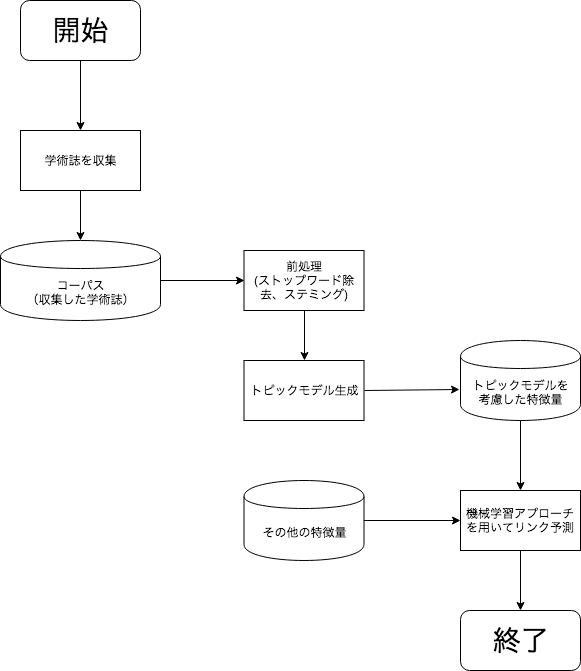
\includegraphics[width = 130mm]{img/diagram.png}
\caption{提案手法のフローチャート}
\label{fig:diagram}
\end{figure}

\chapter{評価\label{valid}}
本章では評価結果を示す。 まず、第\ref{dataset}節で実験に用いるデータセットについて述べる。 第\ref{performance-index}節で評価指標について説明し、第\ref{used-method}節で実験で用いた既存手法について説明する。 第\ref{experimental-method}節で評価方法について説明したあと、第\ref{experimental-result}節で実験結果を示し、第\ref{freedman-valid}節でフリードマン検定とボンフェローニ法による多重比較検定を用いた評価について示す。 さらに、第\ref{importance-feature}節で特徴量の重要度についての評価を示す。
%\ref{importance-feature}節で本実験で用いた特徴量の重要度についての評価を示す。
最後に、これらの結果を踏まえて第\ref{discussion}節で提案手法について議論し、第\ref{future-works}節で今後の課題について述べる。
\section{データセット\label{dataset}}
本研究では、{\it STRING}\cite{STRING17}と呼ばれるタンパク質間相互作用に関するデータベースから、ランダムに3000個のタンパク質の情報を抽出して実験を行なった。 ただし、今回扱ったタンパク質は、ホモ・サピエンスに関するものである。 まず、{\it STRING}から、各タンパク質間の相互作用に関する情報を抽出した。 {\it STRING}から抽出される情報は、各タンパク質間の相互作用が存在するという情報に限るので、未知の相互作用を表現するために、既知の相互作用の$10\%$をランダムに取り除いた。 この$10\%$を未知の相互作用とし、予測することを実験の目的とする。

既知の相互作用を取り除いたあとのタンパク質間相互作用ネットワークを用いて、第\ref{topology-info}項で説明した各タンパク質間の位相的構造から得られる情報や、第\ref{alignment}項、第\ref{gene-ontology}項で説明するタンパク質自身が持つ情報、さらに、提案手法であるトピックモデルを考慮した情報を用いて特徴ベクトルを生成し、精度評価を行なった。 全タンパク質対 ($4498500$対) のうち、$4048650$対(正例 : $119190$対、負例 : $3929460$対)を教師データ、$449850$対(正例 : $13243$対、負例 : $436607$対)をテストデータとして用いた。

今回用いたデータ中のタンパク質が構成するタンパク質間相互作用ネットワークの情報を表 \ref{fig:nw_info}に示す。

\begin{table}[htb]
	\begin{center}
		\caption{タンパク質間相互作用ネットワークの情報}
		\scalebox{0.80}{
		\begin{tabular}{|c|c|c|c|c|c|} \hline
			ノード数 $|V|$ & リンク数 $|E|$ & 平均次数 $c$ & 直径 $|D|$ & 平均パス長 $|L$ & クラスタ係数 $C$ \\ \hline
			3000 & 132433 & 88.29 & 6 & 2.46 & 0.30 \\ \hline
		\end{tabular}
		}
		\label{fig:nw_info}
	\end{center}
\end{table}
		

\section{評価指標\label{performance-index}}
実験の評価には適合率({\it Precision})と再現率({\it Recall})とそれらの調和平均で与えられる{\it f}値を用いる。
\begin{comment}
	のマイクロ平均$micro\mathchar`-f$値を用いる。$micro\mathchar`-f$値は適合率($Precision$)のマイクロ平均($micro\mathchar`-Precision$)と再現率($Recall$)のマイクロ平均($micro\mathchar`-Recall$)の調和平均であり、
\end{comment}
適合率は、正と予測したデータのうち、実際に正であるものの割合、再現率は実際に正であるもののうち、正であると予測されたものの割合を示す。例えば、クラス$C$に対する結果が表 \ref{fig:class}のように得られているとする。ここで$C$に属すると予測したもののうち、$C$に属しているものの数を$a$、$C$に属すると予測したもののうち、$C$に属していないものの数を$b$、$C$に属さないと予測したもののうち、$C$に属しているものの数を$c$、$C$に属していないもののうち、$C$に属していないものの数を$d$で表す。

\begin{table}[tbp]
\begin{center}
\caption{クラス$C$}
\begin{tabular}{|c|c|c|}\hline
&$C$に属する&$C$に属さない\\ \hline
$C$であると予測&$a$&$b$\\ \hline
$C$でないと予測&$c$&$d$\\ \hline
\end{tabular}
\label{fig:class}
\end{center}
\end{table}


この分割結果を下に適合率、再現率、$f$値は次のように定義される。
\begin{equation}
Precision = \frac{a}{a+b}
\end{equation}
\begin{equation}
Recall = \frac{a}{a+c}
\end{equation}
\begin{equation}
f値 = \frac{2 \times Precision \times Recall}{Precision + Recall}
\end{equation}
\begin{comment}
この適合率、再現率、$f$値のマイクロ平均は全クラスの結果を1つにまとめてから評価指標を算出する事で求められる。例えば、クラス$C_{1},C_{2}$に対する結果が以下のように得られているとする。\par
\begin{table}[htb]
\begin{center}
\caption{(a)クラス$C_{1}$}
\begin{tabular}{|c|c|c|}\hline
&$C_{1}$に属する&$C_{1}$に属さない\\ \hline
$C_{1}$であると予測&$a_{1}$&$b_{1}$\\ \hline
$C_{1}$でないと予測&$c_{1}$&$d_{1}$\\ \hline
\end{tabular}
\end{center}
\end{table}
\begin{table}[htb]
\begin{center}
\caption{(b)クラス$C_{2}$}
\begin{tabular}{|c|c|c|}\hline
&$C_{2}$に属する&$C_{2}$に属さない\\ \hline
$C_{2}$であると予測&$a_{2}$&$b_{2}$\\ \hline
$C_{2}$でないと予測&$c_{2}$&$d_{2}$\\ \hline
\end{tabular}
\end{center}
\end{table}
これらの表の各セルの値を足し合わせ、次のように一つの新たな表を作る。\par
\begin{table}[H]
\begin{center}
\caption{(c)表4.2と表4.3を統合した表}
\begin{tabular}{|c|c|c|}\hline
&各クラスに属する&各クラスに属さない\\ \hline
各クラスであると予測&$a_{1}+a_{2}$&$b_{1}+b_{2}$\\ \hline
各クラスでないと予測&$c_{1}+c_{2}$&$d_{1}+d_{2}$\\ \hline
\end{tabular}
\end{center}
\end{table}
この表に対し評価指標の定義式を用いて算出される値が、それぞれの評価指標のマイクロ平均である。
\begin{equation}
micro\mathchar`-Precision = \frac{(a_{1} + a_{2})}{(a_{1} + a_{2}) + (b_{1} + b_{2})}
\end{equation}
\begin{equation}
micro\mathchar`-Recall = \frac{(a_{1} + a_{2})}{(a_{1} + a_{2}) + (c_{1} + c_{2})}
\end{equation}
\begin{equation}
micro\mathchar`-f値 = \frac{2 \times micro\mathchar`-Precision \times micro\mathchar`-Recall}{micro\mathchar`-Precision + micro\mathchar`-Recall}
\end{equation}
\end{comment}
\section{実験で用いた既存手法\label{used-method}}
本節では、実験で用いた既存手法の特徴量の説明をする。 第\ref{alignment}項でタンパク質のアミノ酸配列におけるアライメントを用いた情報について説明し、第\ref{gene-ontology}項で遺伝子オントロジーの情報を考慮した情報について説明する。
\subsection{タンパク質のアミノ酸配列におけるアライメント\label{alignment}}
バイオインフォマティクスにおける基本原理として、アミノ酸配列が似ていれば機能も似ている傾向にある。 その基本原理に基づいて用いられる技術の一つに最適アライメントがある。 最適アライメントとは、可能なアライメントの中でスコアが最大なものを求める手法である。 タンパク質が持つアミノ酸配列を1つの文字列として考えることで、タンパク質の類似性を定量的に算出することを可能にする。 可能なアライメントの数は指数個存在するので、全てのアライメントに対するスコアを算出するためには指数時間必要である。 そこで動的計画法を用いて最大スコアを求めるアルゴリズムが提案された。

動的計画法を用いたアルゴリズムについて説明する。
$F(i, j)$を配列$x_1, x_2, \cdots, x_i$と$y_1, y_2, \cdots, y_j$の最適アライメントのスコアとする。 まず、式 (\ref{eq:init})で初期化する。 $gap$はギャップペナルティと呼ばれ、定数で与えられる。

\begin{eqnarray}
	\begin{cases}
		gap = const. \\
		F(0, j) = -j \times gap \\
		F(i, 0) = -i \times gap
	\end{cases}
	\label{eq:init}
\end{eqnarray}

漸化式は式 (\ref{eq:zenkasiki})で与えられる。 $s(x_i, y_j)$とは置換スコア(行列)と呼ばれ、各文字間の類似性を定量化している。 アミノ酸配列に対するスコア行列は、進化の過程における相対的な置換のしやすさを反映している。 代表的な置換スコア行列として、{\it BLOSUM}行列や{\it PAM}行列が用いられているが、本研究では{\it BLOSUM}行列 (図 \ref{fig:BLOSUM62})を用いる。

\begin{eqnarray}
	F(i, j) = \max
	\begin{cases}
		F(i - 1, j - 1) + s(i, j) \\
		F(i - 1, j) - gap \\
		F(i, j - 1) - gap
	\end{cases}
	\label{eq:zenkasiki}
\end{eqnarray}

最適アライメントのスコアは、$x_1, x_2, \cdots, x_n$と$y_1, y_2, \cdots, y_m$の2つのアミノ酸配列が与えられた場合、$F(n, m)$の値である。

\begin{figure}[hbt]
	\centering
\includegraphics[width=11cm]{BLOSUM62.png}
	\caption{BLOSUM62}
	\label{fig:BLOSUM62}
\end{figure}
\begin{comment}
\subsection{論文における共起性}
論文における共起性を用いた類似尺度は、タンパク質を構成する遺伝子が共に出現する論文の数をカウントし、その数が多いほど類似度が高いという仮定の下提案されている。 遺伝子$x$が出現する論文の集合を$\Gamma(x)$とすることで集合の類似尺度を適用することができる。 (例:Jaccard's coefficientやOverlap coefficient)
\end{comment}
\subsection{遺伝子オントロジー\label{gene-ontology}}
遺伝子オントロジー ({\it Gene Ontology})とは、遺伝子の生物学的プロセス、細胞の構成要素、分子機能を下に遺伝子に付与されるアノテーションのことである\cite{GO-database}。 遺伝子オントロジーは階層構造を持っており、最上位の階層は以下の3つで分類されている。
\begin{itemize}
	\item {\it Biological Process} (生物学的プロセス)
	\item {\it Cellular Component} (細胞の構成要素)
	\item {\it Molecular Function} (分子機能)
\end{itemize}
遺伝子オントロジーで定義された用語を{\it GO term}と呼び、IDが割り当てられている(例:{\it GO:0004888、GO:0005515})。 遺伝子オントロジーは有効非巡回グラフで表現され、ノードが各{\it GO term}を、リンクがそれらの{\it GO term}に関係があることを示している\cite{Schlicker06}。 つまり、各{\it GO term}は一つ以上の親に相当する{\it GO term}と「$is-a$」、「$part-of$」関係をもつ。

これ以降本項では、本研究で用いる、{\it tf-idf} ({\it Term Frequency-Inverse Document Frecuency}) の考えを用いた類似尺度について説明し、その他の遺伝子オンドロジーに基づく類似尺度については\ref{ref:go-term}節で説明する。

{\it Huang}らは、多くの遺伝子に付与されている{\it GO term}はそれほど重要ではなく、あまり付与されていない{\it GO term}の情報を重要視するために、{\it tf-idf}の考えを用いた類似尺度の提案をした\cite{go-tfidf}。 

{\it Huang}らは有効非巡回グラフ内の全ての用語の寄与を示すために、各用語$t$の先祖ノード集合を以下のように定義した。
\begin{eqnarray}
	EV(t) = \{t^{`} ; t^{`} \in DAG(t)\}
	\label{eq:EV}
\end{eqnarray}
ただし、{\it DAG(t)}は$t$の自分自身と先祖ノードを含む{\it GO term}集合である。

図 \ref{fig:go-dag}に、{\it cell-cell adhesion}が形成する有効非巡回グラフの例を示す。 図 \ref{fig:go-dag}の場合、「{\it cell-cell adhesion (GO 0016337)}」の先祖ノードは「{\it cell adhesion (GO : 0007155)}」、「{\it celluar process (GO : 0009987)}」、「{\it biological adhesion (GO : 0022610)}」、「{\it biological process (GO : 0008150)}」である。 したがって({\it GO:0007155})の先祖ノード集合は、$EV(GO:0007155) = \{GO : 0007155, GO : 0009987, GO : 0022610, GO : 008150\}$となる。

次に、ある遺伝子$G$にアノテーションされているGO termが複数の先祖ノード集合に出現する可能性があるので、その出現頻度の情報を含む集合を次のように定義した。
\begin{eqnarray}
	EA(G) = \{(t, freq) ; t \in G_a\}
	\label{eq:EA}
\end{eqnarray}
ただし、$G_a$は遺伝子$G$にアノテーションされている{\it GO term}とそれらの先祖ノード集合、{\it freq}は$G_a$内における{\it GO term}$t$の出現頻度を表す。 {\it (GO : 0009987)} と {\it (GO : 002610)} がアノテーションされている遺伝子$G$を考えた場合、図 \ref{fig:go-dag}では、{\it (GO : 0008150)}は{\it (GO : 0009087)}と{\it (GO : 0022610)}の先祖ノード集合で出現する。 したがって、$EA(G) = \{(GO : 0009987, 1), (GO : 0022610, 1), (GO : 0008150, 2)\}$となる。

\begin{figure}[hbt]
	\centering
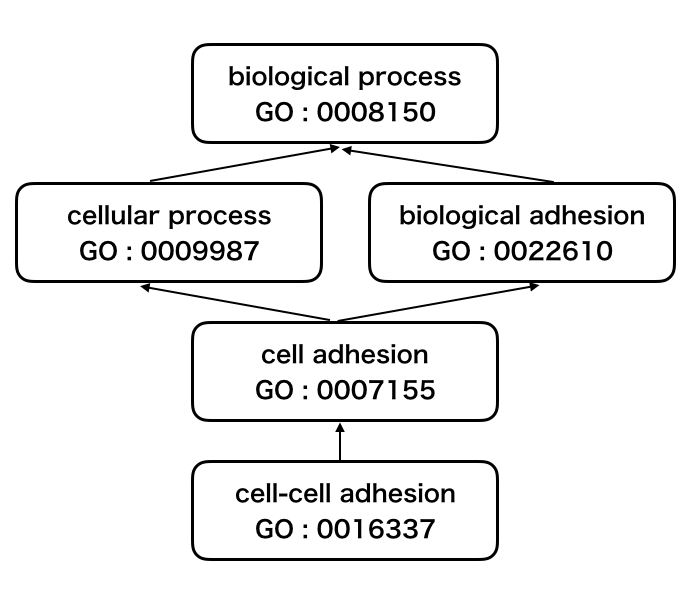
\includegraphics[width=11cm]{img/GO-tfidf.png}
	\caption{{\it cell-cell adhesion (GO:0016337)} が形成する有効非巡回グラフ}
	\label{fig:go-dag}
\end{figure}


最後に、これらの定義された集合 (式 (\ref{eq:EV})や式 (\ref{eq:EA}))に基づいて、遺伝子$G$にアノテーションされている{\it GO term}$t$に対する重みを{\it tf-idf}の考えを考慮し、以下のように計算した。

\begin{eqnarray}
	w_{t,G} = TF_{t,G} \cdot IDF_{t} = \frac{f_{t, G}}{max_{z}f_{t,G}} \ln(\frac{N}{n_t} + 0.01)
\end{eqnarray}
ただし、$f_t$は、式 (\ref{eq:EA})で得られた$EA(G)$における$freq$、$z$は遺伝子$G$にアノテーションされている{\it GO term}の数、$N$はデータセット中の全遺伝子数、$n_t$は{\it GO term}$t$が出現する遺伝子の数である。

遺伝子$G_i$における{\it GO term} $t_i$の重みを$w_{t_i,G_i}$としたとき、$G_i = [w_{t_1, G_i}, $ \par $w_{t_2, G_i}, \cdots, w_{t_n, G_i}]$としてベクトル表現することが可能である。 ただし、ここで$n$はデータセット中に存在する{\it GO term}の総数を表す。

各遺伝子のベクトルを用いて式 (\ref{eq:gene-cosine})で与えられるコサイン類似度を計算することで、遺伝子の類似度を計算する。

\begin{eqnarray}
	sim(G_i, G_j) = \frac{\sum_{k = 1}^{n}w_{t_k, G_i}w_{t_k, G_j}}{\sqrt{\sum_{k = 1}^{n}w^{2}_{t_k, G_i}}\sqrt{\sum_{k = 1}^{n}w^{2}_{t_k, G_j}}}
	\label{eq:gene-cosine}
\end{eqnarray}
コサイン類似度は、$0$から$1$の間の値をとり、$1$に近いほどそれらの遺伝子が類似していることを表す。
\section{評価方法\label{experimental-method}}
トピックモデルを考慮した新規特徴量を組み込むことで、精度向上に貢献することを確認するために、既存の情報 (位相的構造から得られる情報や、タンパク質自身が持つ情報) とのあらゆる組み合わせによって構成される特徴ベクトルを用いて、ランダムフォレスト、K-最近傍法、決定木、サポートベクターマシン、ナイーブベイズ分類器、ロジスティック回帰、ニューラルネットワークの7つの手法で精度評価を行った。 その際、10-分割交差検定を行なった。 その後、フリードマン検定および多重検定を用いて、トピックモデルを考慮した特徴量を含む特徴ベクトルと、その他の特徴ベクトルとの間に有意差があることを確認し、どの特徴ベクトル間に有意差があるかを示す。 さらに、ランダムフォレストを用いて、各特徴量の重要度を算出し、リンク予測における提案手法の重要度の評価を行なった。
%最後に各特徴量の重要度をランダムフォレストを用いて算出し考察を行う。
今回実験で用いた特徴ベクトルを表 \ref{fig:vector}に示す。 ただし、各タンパク質のトピックモデルを生成するために収集した文献は、$PubMed$と呼ばれる医学や生物学の分野に関する学術誌への検索エンジンに掲載されている学術誌のアブストラクトをコーパスとして用いた。 そのあと、前処理として、ストップワードの除去とステミングを行い、{\it LDA}を用いてトピックモデルを生成した。
\begin{table}[tbp]
	\begin{center}
		\caption{実験に用いた特徴ベクトル}
		\begin{tabular}{|c|p{12cm}|} \hline
			$\bm{x}_1$ & {\it topology}\footnotemark \\ \hline
			$\bm{x}_2$ & {\it topology} + {\it alighment}\footnotemark[2] \\ \hline
			$\bm{x}_3$ & {\it topology} + {\it GO}\footnotemark[3]\\ \hline
			%$\bm{x_4}$ & topology + text\footnotemark[4]\\ \hline
			$\bm{x}_4$ & {\it topology} + {\it topic model}\footnotemark[4]\\ \hline
			$\bm{x}_5$ & {\it topology} + {\it alignment} + {\it topic model}\\ \hline
			$\bm{x}_6$ & {\it topology} + {\it GO} + {\it topic model}\\ \hline
			%$\bm{x_8}$ & topology + text + topic model\\ \hline
			$\bm{x}_7$ & {\it topology} + {\it alignment} + {\it GO}\\ \hline
			$\bm{x}_8$ & {\it topology} + {\it alignment} + {\it GO} + {\it topic model}\\ \hline
			%$\bm{x_{11}}$ & topology + alignment + text \\ \hline
			%$\bm{x_{12}}$ & topology + alignment + text + topic model\\ \hline
			%$\bm{x_{13}}$ & topology + alignment + GO + text\\ \hline
			%$\bm{x_{14}}$ & topology + alignment + GO + text + topic model\\ \hline
		\end{tabular}
		\label{fig:vector}
	\end{center}
\end{table}
\footnotetext{位相的構造から得られる情報}
\footnotetext[2]{アミノ酸配列のアライメント}
\footnotetext[3]{遺伝子オントロジーに基づく情報}
%\footnotetext[4]{学術誌における共起性}
\footnotetext[4]{トピックモデル}

\section{実験結果\label{experimental-result}}
表 \ref{fig:conc}に、各特徴ベクトルと、各分類器に対する実験結果を示す。 ただし、表中の{\it RF}はランダムフォレスト、{\it KNN}はK-最近傍法、{\it DT}は決定木、{\it SVM}はサポートベクターマシン、{\it NB}はナイーブベイズ分類器、{\it LR}はロジスティック回帰、{\it NN}はニューラルネットワークを示している。

\begin{table}[H]
	\begin{center}
		\caption{実験結果}
		\begin{tabularx}{120mm}{CCCCC}
			\hline
			\multicolumn{1}{|l|}{特徴ベクトル} &
			\multicolumn{1}{l|}{分類器} &
			\multicolumn{1}{r|}{適合率} &
			\multicolumn{1}{r|}{再現率} &
			\multicolumn{1}{r|}{f値} \\ \hline

			\multicolumn{1}{|l|}{} &
			%\multicolumn{1}{l|}{RF\footnotemark[5]}  &
			\multicolumn{1}{l|}{{\it RF}}  &
			\multicolumn{1}{r|}{0.69} &
			\multicolumn{1}{r|}{0.56} &
			\multicolumn{1}{r|}{0.62} \\ \cline{2-5} 

			\multicolumn{1}{|l|}{} &
			%\multicolumn{1}{l|}{KNN\footnotemark[6]} &
			\multicolumn{1}{l|}{{\it KNN}} &
			\multicolumn{1}{r|}{0.60} &
			\multicolumn{1}{r|}{0.54} &
			\multicolumn{1}{r|}{0.57} \\ \cline{2-5} 

			\multicolumn{1}{|l|}{} &
			%\multicolumn{1}{l|}{DT\footnotemark[7]} & 
			\multicolumn{1}{l|}{{\it DT}} & 
			\multicolumn{1}{r|}{0.70} & 
			\multicolumn{1}{r|}{0.54} &
			\multicolumn{1}{r|}{0.61} \\ \cline{2-5} 

			\multicolumn{1}{|c|}{$\bm{x}_1$} &
			%\multicolumn{1}{l|}{SVM\footnotemark[8]} &
			\multicolumn{1}{l|}{{\it SVM}} &
			\multicolumn{1}{r|}{0.76} &
			\multicolumn{1}{r|}{0.54} &
			\multicolumn{1}{r|}{0.63} \\ \cline{2-5} 

			\multicolumn{1}{|c|}{} &
			%\multicolumn{1}{l|}{NB\footnotemark[9]} &
			\multicolumn{1}{l|}{{\it NB}} &
			\multicolumn{1}{r|}{0.59} &
			\multicolumn{1}{r|}{0.50} &
			\multicolumn{1}{r|}{0.54} \\ \cline{2-5} 

			\multicolumn{1}{|l|}{} &
			%\multicolumn{1}{l|}{LR\footnotemark[10]} &
			\multicolumn{1}{l|}{{\it LR}} &
			\multicolumn{1}{r|}{0.60} &
			\multicolumn{1}{r|}{0.51} &
			\multicolumn{1}{r|}{0.55} \\ \cline{2-5} 

			\multicolumn{1}{|l|}{} &
			%\multicolumn{1}{l|}{NN\footnotemark[11]} &
			\multicolumn{1}{l|}{{\it NN}} &
			\multicolumn{1}{r|}{0.65} &
			\multicolumn{1}{r|}{0.56} &
			\multicolumn{1}{r|}{0.60} \\ \hline \hline

			\multicolumn{1}{|l|}{} &
			\multicolumn{1}{l|}{{\it RF}} &
			\multicolumn{1}{r|}{0.70} &
			\multicolumn{1}{r|}{0.66} &
			\multicolumn{1}{r|}{0.68} \\ \cline{2-5} 

			\multicolumn{1}{|l|}{} &
			\multicolumn{1}{l|}{{\it KNN}} &
			\multicolumn{1}{r|}{0.70} &
			\multicolumn{1}{r|}{0.57} &
			\multicolumn{1}{r|}{0.63} \\ \cline{2-5} 

			\multicolumn{1}{|l|}{} &
			\multicolumn{1}{l|}{{\it DT}} &
			\multicolumn{1}{r|}{0.69} &
			\multicolumn{1}{r|}{0.60} &
			\multicolumn{1}{r|}{0.64} \\ \cline{2-5} 

			\multicolumn{1}{|c|}{$\bm{x}_2$} &
			\multicolumn{1}{l|}{{\it SVM}} &
			\multicolumn{1}{r|}{0.68} &
			\multicolumn{1}{r|}{0.62} &
			\multicolumn{1}{r|}{0.65} \\ \cline{2-5} 

			\multicolumn{1}{|c|}{} &
			\multicolumn{1}{l|}{{\it NB}} &
			\multicolumn{1}{r|}{0.60} &
			\multicolumn{1}{r|}{0.53} &
			\multicolumn{1}{r|}{0.56} \\ \cline{2-5} 

			\multicolumn{1}{|l|}{} &
			\multicolumn{1}{l|}{{\it LR}} &
			\multicolumn{1}{r|}{0.60} &
			\multicolumn{1}{r|}{0.56} &
			\multicolumn{1}{r|}{0.58} \\ \cline{2-5} 

			\multicolumn{1}{|l|}{} &
			\multicolumn{1}{l|}{{\it NN}} &
			\multicolumn{1}{r|}{0.71} &
			\multicolumn{1}{r|}{0.60} &
			\multicolumn{1}{r|}{0.65} \\ \hline \hline

			\multicolumn{1}{|l|}{} &
			\multicolumn{1}{l|}{{\it RF}} &
			\multicolumn{1}{r|}{0.71} &
			\multicolumn{1}{r|}{0.62} &
			\multicolumn{1}{r|}{0.66} \\ \cline{2-5} 

			\multicolumn{1}{|l|}{} &
			\multicolumn{1}{l|}{{\it KNN}} &
			\multicolumn{1}{r|}{0.69} &
			\multicolumn{1}{r|}{0.56} &
			\multicolumn{1}{r|}{0.62} \\ \cline{2-5} 

			\multicolumn{1}{|l|}{} &
			\multicolumn{1}{l|}{{\it DT}} &
			\multicolumn{1}{r|}{0.71} &
			\multicolumn{1}{r|}{0.60} &
			\multicolumn{1}{r|}{0.65} \\ \cline{2-5} 

			\multicolumn{1}{|c|}{$\bm{x}_3$} &
			\multicolumn{1}{l|}{{\it SVM}} &
			\multicolumn{1}{r|}{0.68} &
			\multicolumn{1}{r|}{0.64} &
			\multicolumn{1}{r|}{0.66} \\ \cline{2-5} 

			\multicolumn{1}{|c|}{} &
			\multicolumn{1}{l|}{{\it NB}} &
			\multicolumn{1}{r|}{0.61} &
			\multicolumn{1}{r|}{0.53} &
			\multicolumn{1}{r|}{0.57} \\ \cline{2-5} 

			\multicolumn{1}{|l|}{} &
			\multicolumn{1}{l|}{{\it LR}} &
			\multicolumn{1}{r|}{0.64} &
			\multicolumn{1}{r|}{0.55} &
			\multicolumn{1}{r|}{0.59} \\ \cline{2-5} 

			\multicolumn{1}{|l|}{} &
			\multicolumn{1}{l|}{{\it NN}} &
			\multicolumn{1}{r|}{0.69} &
			\multicolumn{1}{r|}{0.65} &
			\multicolumn{1}{r|}{0.67} \\ \hline

			&                       &                       &                       &

		\end{tabularx}
		\label{fig:conc}
	\end{center}
\end{table}


\begin{table}[tbp]
	\begin{center}
		\begin{tabularx}{120mm}{CCCCC}
			\hline
			\multicolumn{1}{|l|}{特徴ベクトル} &
			\multicolumn{1}{l|}{分類器} &
			\multicolumn{1}{r|}{適合率} &
			\multicolumn{1}{r|}{再現率} &
			\multicolumn{1}{r|}{f値} \\ \hline


			\multicolumn{1}{|l|}{} &
			\multicolumn{1}{l|}{{\it RF}} &
			\multicolumn{1}{r|}{0.70} &
			\multicolumn{1}{r|}{0.64} &
			\multicolumn{1}{r|}{0.67} \\ \cline{2-5} 

			\multicolumn{1}{|l|}{} &
			\multicolumn{1}{l|}{{\it KNN}} &
			\multicolumn{1}{r|}{0.65} &
			\multicolumn{1}{r|}{0.59} &
			\multicolumn{1}{r|}{0.62} \\ \cline{2-5} 

			\multicolumn{1}{|l|}{} &
			\multicolumn{1}{l|}{{\it DT}} &
			\multicolumn{1}{r|}{0.71} &
			\multicolumn{1}{r|}{0.6} &
			\multicolumn{1}{r|}{0.65} \\ \cline{2-5} 

			\multicolumn{1}{|c|}{$\bm{x}_4$} &
			\multicolumn{1}{l|}{{\it SVM}} &
			\multicolumn{1}{r|}{0.74} &
			\multicolumn{1}{r|}{0.64} &
			\multicolumn{1}{r|}{0.69} \\ \cline{2-5} 

			\multicolumn{1}{|c|}{} &
			\multicolumn{1}{l|}{{\it NB}} &
			\multicolumn{1}{r|}{0.60} &
			\multicolumn{1}{r|}{0.56} &
			\multicolumn{1}{r|}{0.58} \\ \cline{2-5} 

			\multicolumn{1}{|l|}{} &
			\multicolumn{1}{l|}{{\it LR}} &
			\multicolumn{1}{r|}{0.63} &
			\multicolumn{1}{r|}{0.57} &
			\multicolumn{1}{r|}{0.60} \\ \cline{2-5} 

			\multicolumn{1}{|l|}{} &
			\multicolumn{1}{l|}{{\it NN}} &
			\multicolumn{1}{r|}{0.75} &
			\multicolumn{1}{r|}{0.64} &
			\multicolumn{1}{r|}{0.69} \\ \hline \hline
%
%			&                       &                       &                       &
%
%		\end{tabularx}
%		\label{fig:conc}
%	\end{center}
%\end{table}
%
%
%\begin{table}[!h]
%	\begin{center}
%		\begin{tabularx}{120mm}{CCCCC}
%			\hline
%			\multicolumn{1}{|l|}{特徴量} &
%			\multicolumn{1}{l|}{分類器} &
%			\multicolumn{1}{r|}{適合率} &
%			\multicolumn{1}{r|}{再現率} &
%			\multicolumn{1}{r|}{f値} \\ \hline

			\multicolumn{1}{|l|}{} &
			\multicolumn{1}{l|}{{\it RF}} &
			\multicolumn{1}{r|}{0.75} &
			\multicolumn{1}{r|}{0.59} &
			\multicolumn{1}{r|}{0.66} \\ \cline{2-5} 

			\multicolumn{1}{|l|}{} &
			\multicolumn{1}{l|}{{\it KNN}} &
			\multicolumn{1}{r|}{0.71} &
			\multicolumn{1}{r|}{0.55} &
			\multicolumn{1}{r|}{0.62} \\ \cline{2-5} 

			\multicolumn{1}{|l|}{} &
			\multicolumn{1}{l|}{{\it DT}} &
			\multicolumn{1}{r|}{0.77} &
			\multicolumn{1}{r|}{0.56} &
			\multicolumn{1}{r|}{0.65} \\ \cline{2-5} 

			\multicolumn{1}{|c|}{$\bm{x}_5$} &
			\multicolumn{1}{l|}{{\it SVM}} &
			\multicolumn{1}{r|}{0.74} &
			\multicolumn{1}{r|}{0.63} &
			\multicolumn{1}{r|}{0.68} \\ \cline{2-5} 

			\multicolumn{1}{|c|}{} &
			\multicolumn{1}{l|}{{\it NB}} &
			\multicolumn{1}{r|}{0.63} &
			\multicolumn{1}{r|}{0.52} &
			\multicolumn{1}{r|}{0.57} \\ \cline{2-5} 

			\multicolumn{1}{|l|}{} &
			\multicolumn{1}{l|}{{\it LR}} &
			\multicolumn{1}{r|}{0.63} &
			\multicolumn{1}{r|}{0.55} &
			\multicolumn{1}{r|}{0.59} \\ \cline{2-5} 

			\multicolumn{1}{|l|}{} &
			\multicolumn{1}{l|}{{\it NN}} &
			\multicolumn{1}{r|}{0.71} &
			\multicolumn{1}{r|}{0.65} &
			\multicolumn{1}{r|}{0.68} \\ \hline \hline

			\multicolumn{1}{|l|}{} &
			\multicolumn{1}{l|}{{\it RF}} &
			\multicolumn{1}{r|}{0.73} &
			\multicolumn{1}{r|}{0.62} &
			\multicolumn{1}{r|}{0.67} \\ \cline{2-5} 

			\multicolumn{1}{|l|}{} &
			\multicolumn{1}{l|}{{\it KNN}} &
			\multicolumn{1}{r|}{0.73} &
			\multicolumn{1}{r|}{0.54} &
			\multicolumn{1}{r|}{0.62} \\ \cline{2-5} 

			\multicolumn{1}{|l|}{} &
			\multicolumn{1}{l|}{{\it DT}} &
			\multicolumn{1}{r|}{0.77} &
			\multicolumn{1}{r|}{0.56} &
			\multicolumn{1}{r|}{0.65} \\ \cline{2-5} 


			\multicolumn{1}{|c|}{$\bm{x}_6$} &
			\multicolumn{1}{l|}{{\it SVM}} &
			\multicolumn{1}{r|}{0.74} &
			\multicolumn{1}{r|}{0.65} &
			\multicolumn{1}{r|}{0.69} \\ \cline{2-5} 

			\multicolumn{1}{|c|}{} &
			\multicolumn{1}{l|}{{\it NB}} &
			\multicolumn{1}{r|}{0.63} &
			\multicolumn{1}{r|}{0.54} &
			\multicolumn{1}{r|}{0.58} \\ \cline{2-5} 

			\multicolumn{1}{|l|}{} &
			\multicolumn{1}{l|}{{\it LR}} &
			\multicolumn{1}{r|}{0.65} &
			\multicolumn{1}{r|}{0.56} &
			\multicolumn{1}{r|}{0.60} \\ \cline{2-5} 

			\multicolumn{1}{|l|}{} &
			\multicolumn{1}{l|}{{\it NN}} &
			\multicolumn{1}{r|}{0.74} &
			\multicolumn{1}{r|}{0.65} &
			\multicolumn{1}{r|}{0.69} \\ \hline \hline

			\multicolumn{1}{|l|}{} &
			\multicolumn{1}{l|}{{\it RF}} &
			\multicolumn{1}{r|}{0.71} &
			\multicolumn{1}{r|}{0.60} &
			\multicolumn{1}{r|}{0.65} \\ \cline{2-5} 

			\multicolumn{1}{|l|}{} &
			\multicolumn{1}{l|}{{\it KNN}} &
			\multicolumn{1}{r|}{0.66} &
			\multicolumn{1}{r|}{0.57} &
			\multicolumn{1}{r|}{0.61} \\ \cline{2-5} 

			\multicolumn{1}{|l|}{} &
			\multicolumn{1}{l|}{{\it DT}} &
			\multicolumn{1}{r|}{0.76} &
			\multicolumn{1}{r|}{0.54} &
			\multicolumn{1}{r|}{0.63} \\ \cline{2-5} 

			\multicolumn{1}{|c|}{$\bm{x}_7$} &
			\multicolumn{1}{l|}{{\it SVM}} &
			\multicolumn{1}{r|}{0.69} &
			\multicolumn{1}{r|}{0.65} &
			\multicolumn{1}{r|}{0.67} \\ \cline{2-5} 

			\multicolumn{1}{|c|}{} & 
			\multicolumn{1}{l|}{{\it NB}} &  
			\multicolumn{1}{r|}{0.61} & 
			\multicolumn{1}{r|}{0.52} &
			\multicolumn{1}{r|}{0.56} \\ \cline{2-5} 

			\multicolumn{1}{|l|}{} &
			\multicolumn{1}{l|}{{\it LR}} &
			\multicolumn{1}{r|}{0.62} &
			\multicolumn{1}{r|}{0.53} &
			\multicolumn{1}{r|}{0.57} \\ \cline{2-5} 

			\multicolumn{1}{|l|}{} & 
			\multicolumn{1}{l|}{{\it NN}} &
			\multicolumn{1}{r|}{0.69} & 
			\multicolumn{1}{r|}{0.60} & 
			\multicolumn{1}{r|}{0.64} \\  \hline

			&                       &                       &                       &

		\end{tabularx}
		\label{fig:conc}
	\end{center}
\end{table}


\begin{table}[tbp]
	\begin{center}
		\begin{tabularx}{120mm}{CCCCC}
			\hline
			\multicolumn{1}{|l|}{特徴ベクトル} &
			\multicolumn{1}{l|}{分類器} &
			\multicolumn{1}{r|}{適合率} &
			\multicolumn{1}{r|}{再現率} &
			\multicolumn{1}{r|}{f値} \\ \hline

			\multicolumn{1}{|l|}{} & 
			\multicolumn{1}{l|}{{\it RF}} & 
			\multicolumn{1}{r|}{0.71} & 
			\multicolumn{1}{r|}{0.62} & 
			\multicolumn{1}{r|}{0.66} \\ \cline{2-5} 

			\multicolumn{1}{|l|}{} & 
			\multicolumn{1}{l|}{{\it KNN}} & 
			\multicolumn{1}{r|}{0.69} &  
			\multicolumn{1}{r|}{0.56} &  
			\multicolumn{1}{r|}{0.62} \\ \cline{2-5} 

			\multicolumn{1}{|l|}{} &
			\multicolumn{1}{l|}{{\it DT}} &
			\multicolumn{1}{r|}{0.72} &
			\multicolumn{1}{r|}{0.56} &
			\multicolumn{1}{r|}{0.65} \\ \cline{2-5} 

			\multicolumn{1}{|c|}{$\bm{x}_8$} &
			\multicolumn{1}{l|}{{\it SVM}} &
			\multicolumn{1}{r|}{0.73} &
			\multicolumn{1}{r|}{0.64} &
			\multicolumn{1}{r|}{0.68} \\ \cline{2-5} 

			\multicolumn{1}{|c|}{} &
			\multicolumn{1}{l|}{{\it NB}} &
			\multicolumn{1}{r|}{0.60} &
			\multicolumn{1}{r|}{0.54} &
			\multicolumn{1}{r|}{0.57} \\ \cline{2-5} 

			\multicolumn{1}{|l|}{} &
			\multicolumn{1}{l|}{{\it LR}} &
			\multicolumn{1}{r|}{0.64} &
			\multicolumn{1}{r|}{0.50} &
			\multicolumn{1}{r|}{0.59} \\ \cline{2-5} 

			\multicolumn{1}{|l|}{} &
			\multicolumn{1}{l|}{{\it NN}} &
			\multicolumn{1}{r|}{0.70} &
			\multicolumn{1}{r|}{0.66} &
			\multicolumn{1}{r|}{0.68} \\ \hline

			&                       &                       &                       &

		\end{tabularx}
	\end{center}
\end{table}
%\footnotetext[5]{ランダムフォレスト}
%\footnotetext[6]{K近傍法}
%\footnotetext[7]{決定木}
%\footnotetext[8]{サポートベクターマシーン}
%\footnotetext[9]{ナイーブベイズ分類器}
%\footnotetext[10]{ロジスティック回帰}
%\footnotetext[11]{ニューラルネットワーク}

\section{フリードマン検定と多重比較による評価\label{freedman-valid}}
本節では、まず第\ref{friedman-testing}項で特徴ベクトル間に有意差があることをフリードマン検定を適用して確認し、そのあと第\ref{multiple-comparison}項でどの特徴ベクトル間に有意差が生じているのかをボンフェローニ法による多重比較検定を用いて確認する。 
\subsection{フリードマン検定\label{friedman-testing}}
特徴ベクトル間における精度の差の検定を、フリードマン検定を用いて行なった。 精度は、適合率と再現率の調和平均であるf値を用いた。 フリードマン検定は{\it IBM SPSS Statics}を用いて行なった。 その結果、特徴量ベクトルに有意差が認められた ($p < 0.01$)。
%\begin{comment}
%まずはじめに、帰無仮説$H_0$と対立仮説$H_1$を次のように立てる。
%\begin{itemize}
%	\item 帰無仮説$H_0$ : 特徴量間に差はない
%	\item 帰無仮説$H_1$ : 特徴量間に差がある
%\end{itemize}
%
%次に、各特徴量ごとに精度の小さい順に順位$R_ij$をつける。 ここで言う精度とは、適合率と再現率の調和平均であるf値であり、f値における各特徴量間の差を評価する。 表\ref{tab:feature-f1}が特徴量とf値、表\ref{tab:feature-f1-rank}が順位を示す。
%
%
%\begin{table}[htb]
%	\begin{center}
%		\caption{特徴量とf値}
%		\begin{tabular}{|c||c|c|c|c|c|c|c|c|} \hline
%			分類器 & $\bm{x_1}$ & $\bm{x_2}$ & $\bm{x_3}$ & $\bm{x_4}$ & $\bm{x_5}$ & $\bm{x_6}$ & $\bm{x_7}$ & $\bm{x_8}$ \\ \hline \hline
%			RF & 0.62 & 0.68 & 0.66 & 0.68 & 0.70 & 0.69 & 0.68 & 0.71 \\ \hline
%			SVM & 0.63 & 0.65 & 0.67 & 0.66 & 0.68 & 0.71 & 0.70 & 0.71 \\ \hline
%			NB & 0.54 & 0.56 & 0.56 & 0.57 & 0.59 & 0.59 & 0.56 & 0.58 \\ \hline
%			LR & 0.55 & 0.58 & 0.56 & 0.57 & 0.61 & 0.59 & 0.60 & 0.60 \\ \hline
%			NN & 0.60 & 0.67 & 0.67 & 0.69 & 0.69 & 0.71 & 0.65 & 0.69 \\ \hline
%		\end{tabular}
%		\label{tab:feature-f1}
%	\end{center}
%\end{table}
%
%\begin{table}[htb]
%	\begin{center}
%		\caption{特徴量と精度の順位}
%		\begin{tabular}{|c||c|c|c|c|c|c|c|c|} \hline
%			分類器 & $\bm{x_1}$ & $\bm{x_2}$ & $\bm{x_3}$ & $\bm{x_4}$ & $\bm{x_5}$ & $\bm{x_6}$ & $\bm{x_7}$ & $\bm{x_8}$ \\ \hline \hline
%			RF & 8 & 5 & 7 & 5 & 2 & 3 & 5 & 1 \\ \hline
%			SVM & 8 & 7 & 5 & 6 & 4 & 1.5 & 3 & 1.5 \\ \hline
%			NB & 8 & 6 & 6 & 4 & 1.5 & 1.5 & 6 & 3 \\ \hline
%			LR & 8 & 5 & 7 & 6 & 1 & 4 & 2.5 & 2.5 \\ \hline
%			NN & 8 & 5.5 & 5.5 & 3 & 3 & 1 & 7 & 3 \\ \hline
%		\end{tabular}
%		\label{tab:feature-f1-rank}
%	\end{center}
%\end{table}
%
%表\ref{tab:feature-f1-rank}を下に、各特徴量ごとに順位の和と、順位の2乗和を式(2.20)、(2.21)で計算する。 その結果が表 \ref{tab:feature-f1-rank-sum}である。
%
%最後に、表\ref{tab:feature-f1-rank-sum}の値を、式(2.22)に代入して検定統計量を計算する。 今回の検定統計量は、$\chi^{2}(7) = 26.5$ ($p < 0.01$)である。 したがって、特徴量間の精度をカイ2乗検定を用いて検定した結果、有意差が認められた ($p < 0.01$)。
%\end{comment}

%$\chi^{2}$分布表によると、$\chi^{2}(7)_{0.05} = 14.0671$であるので、帰無仮説$H_0$は有意水準$\alpha = 0.05$で棄却される。 したがって、「特徴量間に精度の差がある ($p < 0.05$)」という結果が得られた。

%\begin{comment}
%\begin{table}[htb]
%	\begin{center}
%		\caption{特徴量と精度の順位の和と2乗和}
%		\begin{tabular}{|c||c|c|c|c|c|c|c|c|} \hline
%			分類器 & $\bm{x_1}$ & $\bm{x_2}$ & $\bm{x_3}$ & $\bm{x_4}$ & $\bm{x_5}$ & $\bm{x_6}$ & $\bm{x_7}$ & $\bm{x_8}$ \\ \hline \hline
%			RF & 8 & 5 & 7 & 5 & 2 & 3 & 5 & 1 \\ \hline
%			SVM & 8 & 7 & 5 & 6 & 4 & 1.5 & 3 & 1.5 \\ \hline
%			NB & 8 & 6 & 6 & 4 & 1.5 & 1.5 & 6 & 3 \\ \hline
%			LR & 8 & 5 & 7 & 6 & 1 & 4 & 2.5 & 2.5 \\ \hline
%			NN & 8 & 5.5 & 5.5 & 3 & 3 & 1 & 7 & 3 \\ \hline
%			NN & 8 & 5.5 & 5.5 & 3 & 3 & 1 & 7 & 3 \\ \hline
%			$R_{\wa j}$ & 40.0 & 28.5 & 30.5 & 24.0 & 11.5 & 11.0 & 23.5 & 11.0 \\ \hline
%			$R^{2}_{\wa j}$ & 1600.0 & 812.25 & 930.25 & 576.0 & 132.25 & 121.0 & 552.25 & 121.0 \\ \hline
%
%		\end{tabular}
%		\label{tab:feature-f1-rank-sum}
%	\end{center}
%\end{table}
%\end{comment}

\subsection{多重比較\label{multiple-comparison}}
第\ref{friedman-testing}項で特徴ベクトル間に差があるという結果が得られたので、どの特徴ベクトル間に有意差があるのかを、多重比較で確認した。 多重比較は、{\it IBM SPSS Statics}を用いて行なった。 すべての対比較を行う際に有意水準を調整するために、ボンフェローニ法による多重比較検定を行なった。 {\it IBM SPSS Statics}を用いて求めた各特徴ベクトル対の調整済み有意確率と検定結果を表 \ref{tab:feature-conc}に示す。 上三角の部分が、各特徴ベクトル対における調整済みの有意確率であり、下三角の部分が、検定結果である。  また、各特徴ベクトルの精度に関する箱ひげ図を図 \ref{fig:hakohige}に示す。

%\begin{comment}
%まず、帰無仮説と対立仮説を以下のようにたてる。
%\begin{itemize}
%	\item 帰無仮説$H_0$ : 各特徴量間に差はない
%	\item 対立仮説$H_1$ : 各特徴量間に差がある
%\end{itemize}
%
%次に、表\ref{tab:feature-f1-rank-sum}の値を式(2.23)、(2.24)に代入して、各特徴量ごとの平均順位$\bar{R}_{\wa j}$と分散$V$を計算する。 平均順位を計算した結果、表\ref{tab:feature-f1-rank-mean}が得られる。 また分散は$V = 202.0$である。
%
%\begin{table}[htb]
%	\begin{center}
%		\caption{特徴量と精度の順位の平均}
%		\begin{tabular}{|c||c|c|c|c|c|c|c|c|} \hline
%			分類器 & $\bm{x_1}$ & $\bm{x_2}$ & $\bm{x_3}$ & $\bm{x_4}$ & $\bm{x_5}$ & $\bm{x_6}$ & $\bm{x_7}$ & $\bm{x_8}$ \\ \hline \hline
%			RF & 8 & 5 & 7 & 5 & 2 & 3 & 5 & 1 \\ \hline
%			SVM & 8 & 7 & 5 & 6 & 4 & 1.5 & 3 & 1.5 \\ \hline
%			NB & 8 & 6 & 6 & 4 & 1.5 & 1.5 & 6 & 3 \\ \hline
%			LR & 8 & 5 & 7 & 6 & 1 & 4 & 2.5 & 2.5 \\ \hline
%			NN & 8 & 5.5 & 5.5 & 3 & 3 & 1 & 7 & 3 \\ \hline \hline
%			$\bar{R}_{\wa j}$ & 8.0 & 5.7 & 6.1 & 4.8 & 2.3 & 2.2 & 4.7 & 2.2 \\ \hline
%		\end{tabular}
%		\label{tab:feature-f1-rank-mean}
%	\end{center}
%\end{table}
%\end{comment}

多重比較の結果、位相的特性から得られる情報に加えトピックモデルを付加した特徴ベクトル$\bm{x}_4$と$\bm{x}_1$との間に有意差が認められた($p < 0.01$)。 その他に、$\bm{x}_2$、$\bm{x}_7$との間にも有意差が認められた$(p < 0.05)$。 いずれも、トピックモデルを考慮していない特徴ベクトルとの間に有意差が確認できた。

その他に$\bm{x}_1$と$\bm{x}_3$、$\bm{x}_1$と$\bm{x}_6$、$\bm{x}_1$と$\bm{x}_8$、$\bm{x}_2$と$\bm{x}_6$、$\bm{x}_6$と$\bm{x}_7$との間に有意差が認められた($p < 0.05$)。 また$\bm{x}_1$と$\bm{x}_5$との間に有意差が認められた($p < 0.01$)。

\begin{table}[tbp]
	\begin{center}
		\caption{各特徴ベクトル対の調整済み有意確率と検定結果}
		\scalebox{0.85} {
			\begin{tabular}{|c||c|c|c|c|c|c|c|c|} \hline
				特徴ベクトル & $\bm{x}_1$ & $\bm{x}_2$ & $\bm{x}_3$ & $\bm{x}_4$ & $\bm{x}_5$ & $\bm{x}_6$ & $\bm{x}_7$ & $\bm{x}_8$ \\ \hline \hline
				$\bm{x}_1 $ &  & 1.000 & {\bf 0.036} & {\bf $<$ 0.001} & {\bf 0.036} & {\bf $<$ 0.001} & 1.000 & {\bf 0.036} \\ \hline
				$\bm{x}_2 $ & n.s. &  & 0.934 & {\bf 0.016} & 0.934 & {\bf 0.016} & 1.000 & 0.934 \\ \hline
				$\bm{x}_3 $ & * & n.s. &  & 1.000 & 0.615 & 1.000 & 1.000 & 1.000 \\ \hline
				$\bm{x}_4 $ & ** & * & n.s. &  & 1.000 & 1.000 & {\bf 0.020} & 1.000 \\ \hline
				$\bm{x}_5 $ & * & n.s. & n.s. & n.s. &  & 1.000 & 1.000 & 1.000 \\ \hline
				$\bm{x}_6 $ & ** & * & n.s. & n.s. & n.s. &  & {\bf 0.020} & 1.000 \\ \hline
				$\bm{x}_7 $ & n.s. & n.s. & n.s. & * & n.s. & * &  & 1.000 \\ \hline
				$\bm{x}_8 $ & * & n.s. & n.s. & n.s. & n.s. & n.s. & n.s. & \\ \hline
			\end{tabular}
		}
		\\n.s. : 非有意、 * : 有意($p < 0.05$), ** : 有意($p < 0.01$)
		\label{tab:feature-conc}
	\end{center}
\end{table}


\begin{figure}[htbp]
	\begin{center}
	\caption{特徴ベクトルとf値の箱ひげ図}
		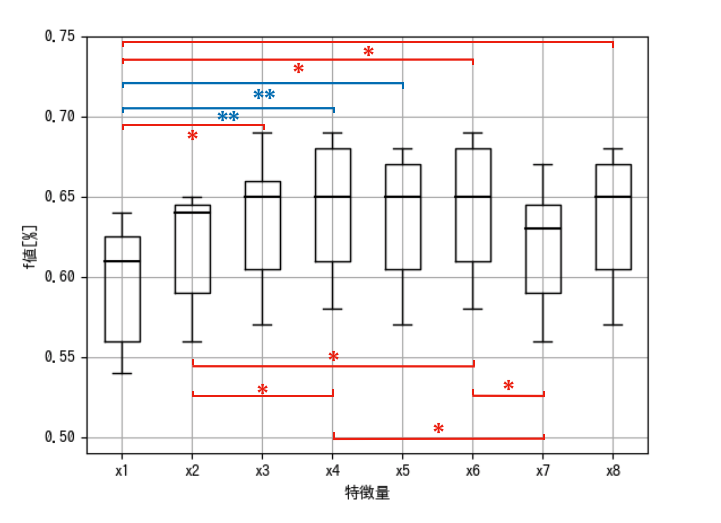
\includegraphics[width = 102mm]{img/feature-hakohige2.png}
	\label{fig:hakohige}
	\\ * : 有意($p < 0.05$), ** : 有意($p < 0.01$)
	\end{center}
\end{figure}

%特徴量$i$と特徴量$j$の対比較のための検定統計量$S_{ij}$を式(2.25)を用いて計算する。 今回の統計量$S_{ij}$は自由度7の$\chi^{2}$分布に従う。 表\ref{tab:feature-f1-rank-mean}と分散$V = 202.0$を下に、各特徴量対の検定統計量を計算した結果が表\ref{tab:feature-conc}の上三角形の部分である。 表\ref{tab:feature-conc}に示した検定統計量は全て自由度7の$\chi^{2}$分布に従うので、有意水準$\alpha = 0.05$に対して、$\chi^{2}(7) > \chi^{2}_{0.05}(7)$ならば帰無仮説$H_0$は棄却され、$\chi^{2}(7) \leq \chi^{2}_{0.05}(3)$ならば帰無仮説$H_0$は棄却されない。 今回自由度7の$\chi^{2}$分布表において、$\chi^{2}_0.05(7) = 14.0671$なので、$\bm{x_1}$と$\bm{x_4}$、$\bm{x_1}$と$\bm{x_5}$、$\bm{x_1}$と$\bm{x_7}$に差があるといえ、その他の特徴量間には差があるとはいえないという結論が得られた($p < 0.05$)。


\section{特徴量の重要度の評価\label{importance-feature}}
各特徴量を比較するために、ランダムフォレストを用いて特徴量の重要度を算出した。 その結果が図 \ref{fig:feature-importance}である。 各特徴量の重要度は0から1の間の値をとり、総和が1となるように算出する。 重要度が1に近いほど重要度の高い特徴量であることを表す。

{\it Jaccard's coefficient}が、最大の重要度となった(重要度 = $0.150$)。 続いて、提案手法であるトピックモデルが重要であるという結果が得られた (重要度$ = 0.143$)。 その次に、{\it Sorensen Dice coefficient}、遺伝子オントロジーという順で重要であると判断できる (それぞれ、重要度$ = 0.121$、重要度 = $0.120$)。 一方で、アミノ酸配列のアライメント情報は、2番目に低い重要度となった (重要度$ = 0.060$)。 これらの結果から、今回の実験において、トピックモデルを考慮した特徴量は、分類をする上で重要な情報源となっていると考える。
% cn     jc   AAI   PA    RAI   DSC   over  amino  GO    topic
%0.090 0.150 0.075 0.105 0.083 0.123 0.045 0.060 0.120 0.143

\begin{figure}[htbp]
	\begin{center}
	\caption{特徴量の重要度}
		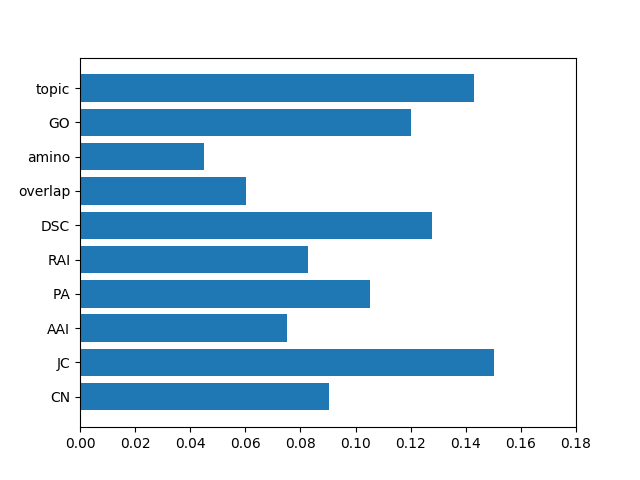
\includegraphics[width = 103mm]{img/feature_importance.png}
	\label{fig:feature-importance}
		\\ {\footnotesize CN : {\it common neighbors}、JC : {\it JAccard's coefficient}、AAI : {\it Adamic/Adar index}、\\PA : {\it Prefential attachment}、RAI : {\it Resource allocation}、DSC : {\it Sorensen dice coefficient}、overlap : {\it Overlap coefficient}、 amino : アミノ酸配列のアライメント、\\GO : 遺伝子オントロジー、topic : トピックモデル}
	\end{center}
\end{figure}

\section{議論\label{discussion}}
多重比較検定の結果、$\bm{x}_1$と$\bm{x}_4$との間に有意差が認められたことから、位相的特性から得られる情報に、提案手法であるトピックモデルを付加することで、タンパク質間の表現力を高め、精度向上に貢献できると考える。 さらに、既存手法と提案手法を組み合わせて構成される、$\bm{x}_5$や$\bm{x}_6$、$\bm{x}_8$に関しても、$\bm{x}_1$と有意差が認められたことから、表現力を高め精度向上に貢献できると考えることができる。

また、今回の実験では、遺伝子オントロジーを考慮した特徴ベクトルである$\bm{x}_3$も$\bm{x}_1$と有意差が認められた。  したがって、今回の実験では、遺伝子オントロジーも位相的特性から得られる情報に加えることで、表現力を高めることができると考える。 しかし、アミノ酸配列を新規情報で追加した特徴ベクトルである$\bm{x}_7$は$\bm{x}_1$との間に有意差が認められなかったのに対して、アミノ酸配列をトピックモデルに追加した特徴ベクトルである$\bm{x}_5$は$\bm{x}_1$と有意差があることから、トピックモデルは単体のみならず、他の情報と共に利用する際にも表現力を高めることができると考える。

さらに、特徴量の重要度の評価を行なった結果から、トピックモデルを考慮した特徴量が、分類において重要な情報源であると考えることができる。 このことからも、トピックモデルを考慮した特徴量が、タンパク質対の表現力を高めることができると考える。

\section{今後の課題\label{future-works}}
本研究では、{\it STRING}と呼ばれるデータセットを用いて実験を行ない、本手法の有用性を確認した。 今後は、複数のデータセットにおいて本手法が有用であるかを評価し、汎用性を確認する必要がある。 さらに、今回用いた遺伝子オントロジーやアミノ酸配列の情報の他にも、遺伝子発現の情報\cite{gene-expression08}、比較ゲノムベースの手法\cite{hikaku09}、コドンベースの類似尺度\cite{codon08}、さらに、本手法とは別の、自然言語処理 ({\it natural language processing})やテキストマイニングの技術を用いて抽出される意味的情報\cite{txt-mining10}など、様々な既存手法との比較や、組み合わせによる精度評価を行う必要がある。



%未知のタンパク質間相互作用を予測する研究は、分類アルゴリズムの提案、新規の特徴量の提案の2つに大別される。 分類アルゴリズムの提案は、ベイズ的手法を用いたアルゴリズム、アミノ酸配列を用いたアルゴリズム、リンク予測を用いたアルゴリズム、サポートベクタマシンやランダムフォレストなど数多くの機械学習の手法を用いたアルゴリズムなどが提案されている。 一方、新規の特徴量では、タンパク質の構造から抽出する方法、タンパク質間相互作用ネットワークから位相的情報を抽出する手法や、論文や学術誌などから自然言語処理 (natural language processing) やテキストマイニングの技術を用いて意味的情報を抽出する手法などが提案されている。
%$\bm{x_4}$と有意差があることからトピックモデルを考慮した特徴量の方がより精度向上に貢献できると考える。 また、$\bm{x_6}$との間にも有意差があることから、トピックモデルは単体のみならず、他の情報と共に使用する際にも表現力を高めることができると考える。

\chapter{関連研究\label{reference}}
\section{決定木}
決定木は、データの分類を繰り返し行い、分岐過程を階層化して木で表現される。 現在、広く使われている{\it CART} ({\it Classification and Regression Tree}) 法は{\it Breiman}らによって提案された\cite{decision-tree}。 {\it CART}法は、分類のみならず、回帰に対しても適用することができるアルゴリズムである。

繰り返しデータを分割し、徐々にデータを分類していくが、データを分割するためには基準が必要である。 {\it CART}法ではいくつかの基準が提案されているが、一般に広く使われているのはジニ係数である。 ジニ係数は、経済の領域で所得格差を表すのに用いられている指標であり、0から1の間の値を取り、0に近いほど平等であることを表す。 各分岐で、偏りが少ないほど、分岐が少ない決定木を構築することができるので、ジニ係数がもっとも低下するように分割していく。 その他にもエントロピーに基づく分類法がある。

\section{ランダムフォレスト}
ランダムフォレスト ({\it random forest}) は、{\it Leo}らによって提案されたアンサンブル学習 ({\it ensemble learning}) の一種である\cite{random}。

ランダムフォレストは、複数の決定木を組み合わせて森 ({\it forest}) を構築することで識別、分類を行う。 個々に学習した複数の学習モデル (決定木) を組み合わせる事で汎化能力を向上させ、一つの学習モデルを作成する。 これはアンセンブル学習と呼ばれ、一つ一つの決定木は、アンセンブル学習における弱学習モデル ({\it weak classifier}) に相当する。

まず学習データを用いて、複数の決定木を構築する。 各決定木は、分岐ノード ({\it Split Node}) と葉ノード ({\it Leaf Node}) により構成され、分岐ノードではそのノードの子のうちどれに進むべきかを決定する分岐関数 ({\it Split Function}) が与えられ、葉には最終的な出力結果が与えられる。
%分岐ノードは
また葉ノードは、そのノードに相当する学習データが持つクラス分布を与える。 識別は、未知データを各決定木に入力し、辿り着いた葉ノードに与えられているクラス分布を出力する。
\section{K最近傍法}
K最近傍法は、回帰や分類を行う際に、類似するデータを{\it K}個集めて多数決的に目的とする値を決定する手法である。 回帰の際には、類似する{\it K}個のデータの平均値や中央値などの値を予測結果とする。 分類のときは、類似する{\it K}個のデータが属するクラスのうち、もっとも数が多いクラスにデータを分類する。 {\it K}はパラメータで、事前に設定する必要がある。

\section{ナイーブベイズ分類器}
ナイーブベイズ分類器 ({\it naive bayes classifier}) は確率に基づいた分類器であり、事例\(X\)に対して\(P(c|X)\)が最大となるクラス\(c \in C\)を出力する。 このとき、ベイズの定理と呼ばれる次の性質を用いる。
\begin{equation}
P(c|X) = \frac{P(c)P(X|c)}{P(X)}
\end{equation}
式(5.1)の右辺を最大にする$c$が、出力となるクラスであるが、分母の\(P(X)\)は\(c\)に依存しないので、最大にする$c_max$は次のように求める。
\begin{equation}
c_{max} = \argmax_{c} \frac{P(c)P(X|c)}{P(X)} = \argmax_{c}P(c)P(X|c)
\end{equation}
ナイーブベイズ分類器は確率分布\(P(X|c)\)にシンプルな分布を仮定する。 事例$X$の正規確率を、正規分布を仮定して表すと、
\begin{equation}
P(X|c) = \prod_{i} P(x_{i}|c) = \prod_{i} \frac{1}{\sqrt{2\pi \sigma^{2}_{c}}}\exp(-\frac{1}{2\sigma^{2}_{c}}(x_{i}-\mu_{c_{i}})^{2})
\end{equation}
となる。 したがって、ナイーブベイズ分類器の正規分布モデルは、
\begin{equation}
P(c)P(X|c) = P(c)\prod_{i} \frac{1}{\sqrt{2\pi \sigma^{2}_{c}}}\exp(-\frac{1}{2\sigma^{2}_{c}}(x_{i}-\mu_{c_{i}})^{2})
\end{equation}
を最大にする\(c\)を出力する。

\section{ロジスティック回帰}
あるデータ$\bm{x}$が与えられたときのクラス$C_1$の事後確率を、
\begin{equation}
	p(C_1 | \bm{x}) = \sigma(\bm{w}^{T}\bm{\phi(x)})
\end{equation}
と表すことができる。 ただし、$\sigma(\cdot)$は式 (\ref{eq:logistic_sigmoid})で定義されるロジスティックシグモイド関数、$\bm{w}$は推定したいパラメータ、$\phi(\cdot)$は基底関数である。 このパラメータの推定方法は様々だが、ここでは最尤法を用いて説明する。

\begin{equation}
	\label{eq:logistic_sigmoid}
	\sigma(x) = \frac{1}{1 + \exp(-x)}
\end{equation}
最尤法なので、ロジスティックシグモイド関数を微分する。 微分をすると、
\begin{equation}
	\frac{d\sigma}{dx} = (1 - \sigma(x))\sigma(x)
\end{equation}
となる。
データの集合 $\{\bm{x_n}, y_n\}$が与えられたときの尤度は、
\begin{eqnarray}
	p(\bm{y}|\bm{w}) &=& \prod_{n = 1}^{N}p(C_1|\bm{\phi(x_n)})^{y_n}p(C_2|\bm{\phi(x_n)})^{1 - y_n}  \nonumber \\
	&=& \prod_{n = 1}^{N} p(C_1|\bm{\phi(x_n)})^{y_n}\{1 - p(C_1|\bm{\phi(x_n)})\}^{1 - y_n} \nonumber \\
	&=& \prod_{n = 1}^{N} \sigma(\bm{w}^{T}\bm{\phi(x_n)}))^{y_n}\{1 - \sigma(\bm{w}^{T}\bm{\phi(x_n)})\}^{1 - y_n}
\end{eqnarray}
と表せる。 ただし、$y_n \in \{0, 1\}$である。 この負の対数尤度を、誤差関数として定義する。
\begin{eqnarray}
	E(\bm{w}) &=& -\log p(\bm{y}|\bm{w}) \nonumber \\
	&=& -\sum_{n = 1}^{N} \{y_n \log \sigma(\bm{w}^{T} \bm{\phi(x_n})) \nonumber \\
	&+& (1 - y_n) \log(1 - \sigma(\bm{w}^{T}\bm{\phi(x_n)}))\}
\end{eqnarray}
この誤差関数$E(\bm{w})$をパラメータ$\bm{w}$で微分し、勾配が0に近くなるようにパラメータを調整していけば良い。 これには、ニュートン法や、勾配降下法などの手法を用いると良い。

\section{ニューラルネットワーク}
ニューラルネットワークは、人間におけるニューロン (神経細胞) の情報伝達の仕組みを模倣したものとして提案された。 脳は、膨大な量のニューロンが集まって構成されていて、ニューロン同士が結合して脳の知的活動を実現している。

ニューラルネットワークでは、ニューロンを数理的にモデル化を行う。 ニューロンは入力を受け取り、式 (\ref{eq:senkeiwa})を用いて値を計算し、その計算結果が設定した閾値を超えたとき、発火したものとみなし、他のニューロンに情報を伝達する。 ニューロンを視覚的に表現したものが、図 \ref{fig:single-perceptron}である。
\begin{equation}
	y_n = b + \sum_{d = 1}^{D} w_{nd}x_d
	\label{eq:senkeiwa}
\end{equation}
ただし、$n$は全部で$N$個のうちの$n$番目のデータを表し、$x_d$は入力の$d$次元目の要素を表す。 便宜上$0$次元目の要素を$1$として定義し、1次元目から$D$次元目がデータ自身が持つ特徴量である。$w_{nd}$は重みであり、$b$はバイアスと呼ばれる。 $y_n$が閾値$\theta$を超えたときに1を、下回ったときに0を返す。 
\begin{figure}[tbp]
	\begin{center}
		\caption{ニューロンのモデル}
		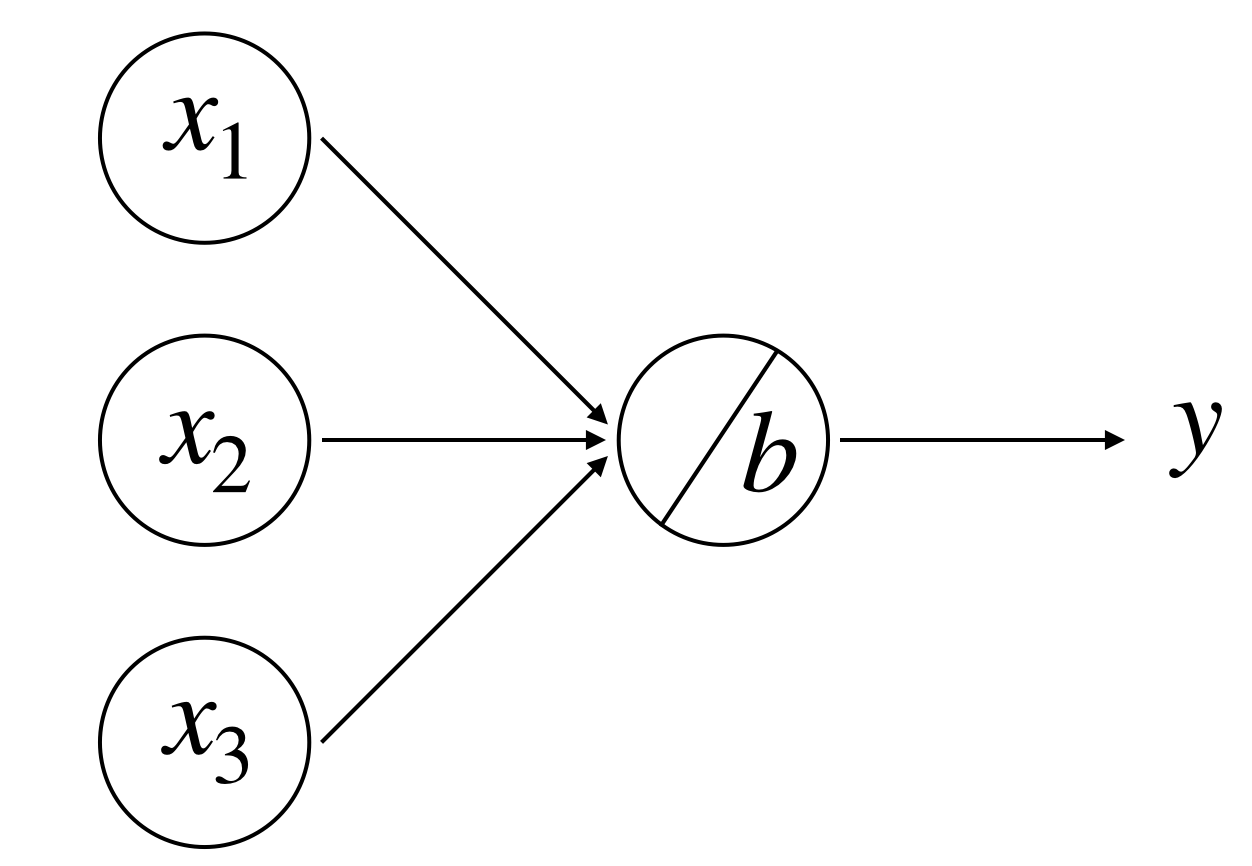
\includegraphics[width = 120mm]{img/single-perceptron.png}
		\label{fig:single-perceptron}
	\end{center}
\end{figure}

ニューラルネットワークは、ある層のニューロンが、次の層のニューロンに連結するように構成されたものである。 2層のニューラルネットワークを視覚的に表現したものが、図 \ref{fig:multi-perceptron}である。
\begin{figure}[tbp]
	\begin{center}
		\caption{2層のニューラルネットワーク}
		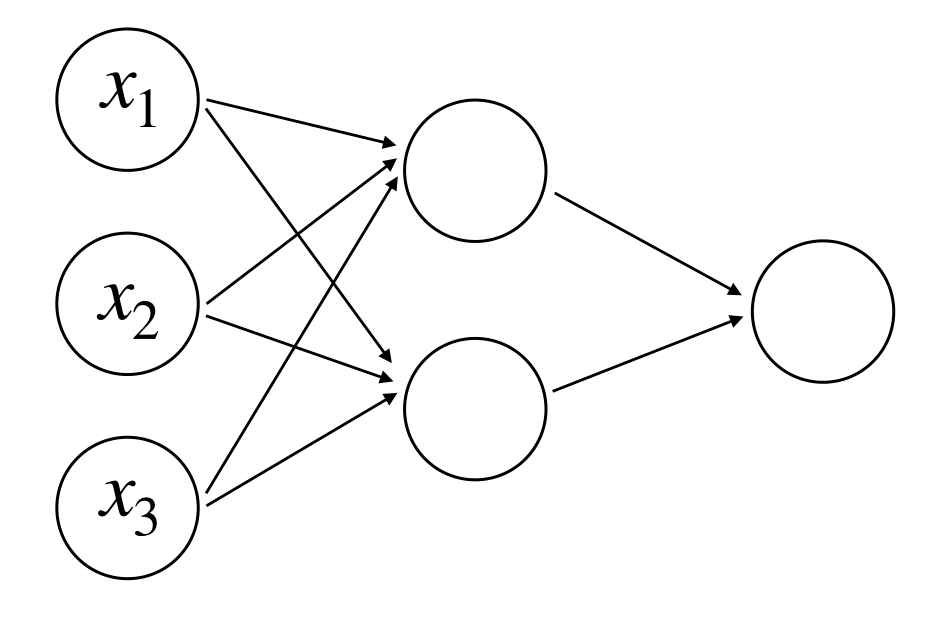
\includegraphics[width = 120mm]{img/multi-perceptron.png}
		\label{fig:multi-perceptron}
	\end{center}
\end{figure}


学習時には、各ニューロン間の重みを出力層側から入力層側に向かって逆方向に調整していく。 この手法をバックプロパゲーション ({\it Backpropagation})と呼ぶ。

さらに、層を重ねることで、様々な目的に適応するモデルを構築することができる。 現在では深層学習 ({\it deep learning}) の研究が盛んであり、画像認識や自動運転、自然言語処理など多様な分野に応用されている。
\begin{comment}

一般的な回帰や、分類器で用いられる線形モデルは、基底関数$\phi$を用いて
\begin{equation}
	\label{linear}
	y(\bm{x}, \bm{w}) = f(\sum w\phi(\bm{x}))
\end{equation}
と表される。 ただし、$f(\cdot)$は回帰では恒等写像、分類器では活性化関数である。 パラメータ$\bm{w}$と基底関数が持つパラメータを同時に調整することが目的である。

基本的なニューラルネットワークも、式 (\ref{linear})と同じ方針をとる。 まず、入力に対する線形和を作る。

ニューラルネットワークは入力データに単に重みづけをして出力しているのではなく、活性化関数を施す。 様々な活性化関数が使われているが、ここではシグモイド関数を用いて説明する。

シグモイド関数は以下のように定義される関数であり、グラフの概形は図 \ref{fig:sigmoid}である。
\begin{eqnarray}
	\sigma(x) = \frac{1}{1 + e^{-x}}
	\label{sigmoid-func}
\end{eqnarray}

\begin{figure}[tbp]
	\begin{center}
	\caption{シグモイド関数}
		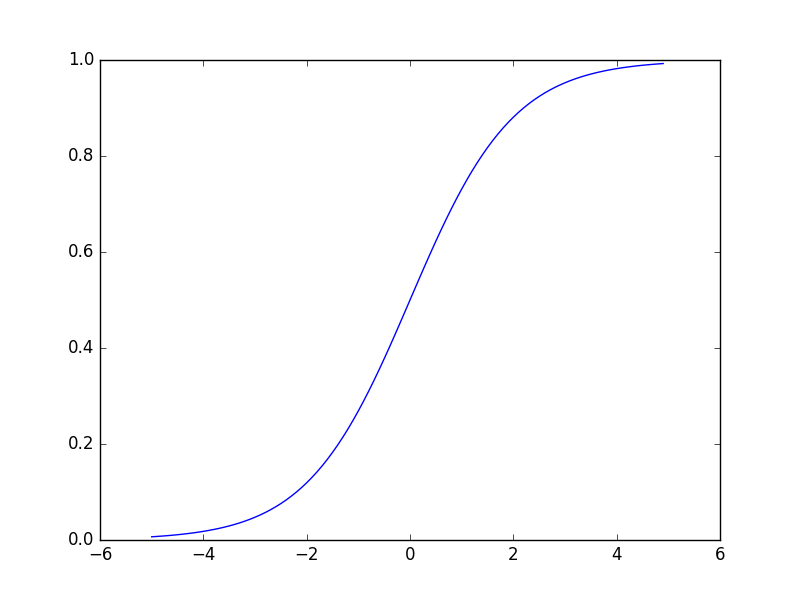
\includegraphics[width = 130mm]{img/sigmoid.png}
	\label{fig:sigmoid}
	\end{center}
\end{figure}

式 (\ref{eq:senkeiwa})の値を$z$とし、その値をシグモイド関数に渡す。

\begin{eqnarray}
	z = b + \sum_{d = 1}^{D} w_{nd}x_d \nonumber \\
	\sigma(z) = \frac{1}{1 + e^{-z}}
	\label{eq:perceptron}
\end{eqnarray}
シグモイド関数は連続的で微分可能な関数であり、その導関数は、
\begin{eqnarray}
	\frac{d\sigma}{dz} = \sigma(z)(1 - \sigma(z))
\end{eqnarray}
である。

式 (\ref{eq:perceptron})を視覚的に表現したものが図 \ref{fig:single-perceptron}であり単一パーセプトロンと呼ばれる。 各入力がニューロンに相当する。
	ここで、最初の層を入力層、真ん中の層を隠れ層、最後の層を出力層と呼ぶ。 計算は式 (\ref{eq:perceptron})を下に、入力層から隠れ層に値が渡され、その値が出力層に対する入力になる。
\end{comment}

\section{遺伝子オントロジーに基づく類似尺度\label{ref:go-term}}
遺伝子オントロジーの階層構造に着目した類似尺度が提案されている。 aに付与された$GO term_a$とbに付与された$GO term_b$の共通の親に相当する$GO term_p$を見つけ、その$GO term_p$が、階層構造の深い位置で定義されているほど、類似度が高いという発想である。 図 \ref{fig:go1}、図 \ref{fig:go2}では{\it GO term}の階層表現の例を表し、赤いノードが、着目している遺伝子に付与された{\it GO term}で、緑のノードが、それらの共通する親のノードである。 図 \ref{fig:go1}の場合、緑のノードの深さが2であることに対し、図 \ref{fig:go2}の場合深さが1である。 したがって、図 \ref{fig:go2}におけるGO term対に比べ、図 \ref{fig:go1}における{\it GO term}対の方が類似度が高いことを表している。 各{\it GO term}対の類似度を算出した後に、その最大値を採用する手法、平均を採用する手法、共通する親の数を採用する手法などが提案されている。 その他にも{\it GO term}対の類似性は、同一の遺伝子にアノテーションされている頻度によっても定義することができる\cite{wu13}。

\begin{figure}[tbp]
	\begin{tabular}{c}
		\begin{minipage}{0.5\hsize}
			\begin{center}
				\includegraphics[width = 3cm, height = 3cm]{fig1.png}
				\caption{例1}
				\label{fig:go1}
			\end{center}
		\end{minipage}

		\begin{minipage}{0.5\hsize}
			\begin{center}
				\includegraphics[width = 3cm, height = 3cm]{fig2.png}
				\caption{例2}
				\label{fig:go2}
			\end{center}
		\end{minipage}
	\end{tabular}
\end{figure}

一つの遺伝子に、複数の{\it GO term}が割当てられていることもあるので、共通して持つ{\it GO term}の数が多いほど、類似度が高いという考え方に基づく類似尺度も提案されている。 例えば、$GO term_i$が付与されている場合、$i$番目の要素を1、割り当てられていない場合は0とするバイナリベクトルを生成し、そのコサイン類似度を遺伝子対の類似尺度とすることもできる。
\begin{comment}
\section{$k$平均法}
$k$平均法($k$-means)と呼ばれる分類手法は、とりあえず適当に事例を分類してから、うまく分類されるように調整して行く事によって分類を行う手法である\cite{kmeans}。クラスタ数$k$はユーザが事前に決めておく必要がある。また、各クラスタは平均ベクトル等の代表ベクトルで表現される。なお、$k$平均法という名称は、$k$個の平均を用いている事を表している。\par
\ex 各ベクトルの次元数を2、クラスタ数$k$が2であるとして、図を用いて説明する。
\\
\begin{screen}
\begin{enumerate}
\item 無作為に代表ベクトルを決める。(図5.4)
\item 各事例ベクトルを一番近い代表ベクトルのクラスタに帰属させる。(図5.5,5.7,5.9)
\item 各クラスタに含まれている事例ベクトルの平均を計算し、それを新たな代表ベクトルとする。(図5.6,5.8,5.10)
\item 2,3を収束する(クラスタに変化がなくなる)まで繰り返し行う(図5.10)
\end{enumerate}
\end{screen}
\begin{figure}[htbp]
\centering
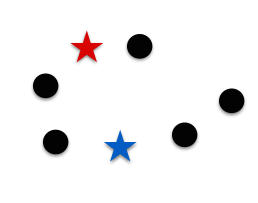
\includegraphics[width = 50mm,bb = 0 0 258 203]{img/knn1.png}
\label{fig:four}
\caption{無作為に代表ベクトルを決める}
\end{figure}
\begin{figure}[htbp]
\centering
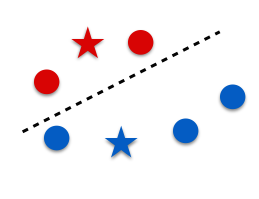
\includegraphics[width = 50mm,bb = 0 0 259 199]{img/knn2.png}
\label{fig:five}
\caption{クラスタの変更}
\end{figure}
\begin{figure}[htbp]
\centering
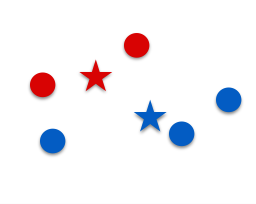
\includegraphics[width = 50mm,bb = 0 0 256 204]{img/knn3.png}
\label{fig:six}
\caption{新たな代表ベクトルを求める}
\end{figure}
\begin{figure}[htbp]
\centering
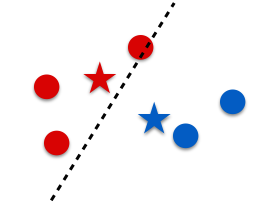
\includegraphics[width = 50mm,bb = 0 0 260 203]{img/knn4.png}
\label{fig:seven}
\caption{クラスタの変更}
\end{figure}
\begin{figure}[htbp]
\centering
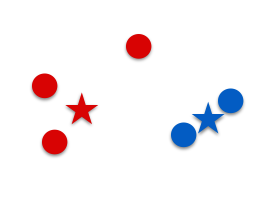
\includegraphics[width = 50mm,bb = 0 0 256 204]{img/knn5.png}
\label{fig:eight}
\caption{新たな代表ベクトルを決める}
\end{figure}
\begin{figure}[htbp]
\centering
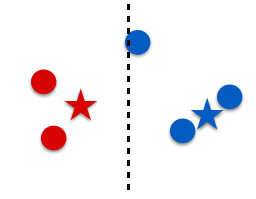
\includegraphics[width = 50mm,bb = 0 0 256 199]{img/knn6.png}
\label{fig:nine}
\caption{クラスタの変更}
\end{figure}
\begin{figure}[htbp]
\centering
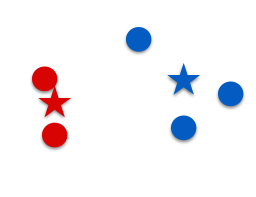
\includegraphics[width = 50mm,bb = 0 0 256 197]{img/knn7.png}
\label{fig:ten}
\caption{新たな代表ベクトルを決める}
\end{figure}
\begin{figure}[htbp]
\centering
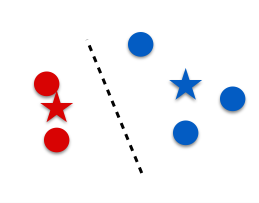
\includegraphics[width = 50mm,bb = 0 0 259 203]{img/knn8.png}
\label{fig:a}
\caption{クラスタリングの終了}
\end{figure}
\newpage
一般の場合についてのk平均法のアルゴリズムは以下のようになる。ただし、$c_{i}$はクラスタ名とそれに対応する集合の両方の意味で用い、関数$sim$は二つのベクトルの類似度を返す。

\begin{algorithm}
	\caption{k平均法}
	\label{algo1}
	\begin{algorithmic}[1]
		 \REQUIRE 事例ベクトル集合$D = \{\bm{x^{(1)}},\bm{x^{(2)}},...,\bm{x^{(|D|)}}\}$,クラスタ数 
		 \STATE 無作為に代表ベクトル$m_{1},m_{2},...,m_{k}$を決定
		 \WHILE{収束}
		   \FOR{$i = 1$ to $|D|$}
		   \STATE $c_{max} = \argmax sim(x^{(i)},m_{c})$\#事例ベクトル集合の分割
		   \STATE $c_{max} \leftarrow x^{(i)}$
		   \ENDFOR
		\STATE $\forall c,\bm{m_{c}} = \frac{1}{|c|}\sum_{\bm{x^{(i)}}\in c}\bm{x^{(i)}}$ \#代表ベクトルを再計算
  \ENDWHILE
 \end{algorithmic}
\end{algorithm}
\end{comment}

\begin{comment}
\section{スペクトラルクラスタリング}
各データをノードとし、それらを結ぶエッジに類似度や距離等に応じて重みを与える事で重みグラフができる。\par
ノード\(V = \{v_{i};i=1,...,n\}\)とデータ\(X=\{x_{i};i=1,...,n\}\)を対応させる。2つのデータ\(x_{i},x_{j}\)の距離や類似度に応じてエッジ\(e_{ij}\)に重み\(w_{ij}\)を与える。このとき、\(W = (w_{ij})\)を重み付き隣接行列と呼ぶ。\par
任意のノード\(v_{i}\in V\)の次数を
\begin{equation}
d_{i} = \sum_{j=1}^{n}w_{ij}
\end{equation}
と定義する。次数を対角成分に持つ\(n\)次正方行列\(D = (\delta_{ij}d_{i})\)を次数行列と呼ぶ。ただし\(\delta_{ij}\)はクロネッカーのデルタである。
\begin{equation}
\delta_{ij} = \begin{cases}
1 & (i = j) \\
0 & (i \neq j)
\end{cases}
\end{equation}
重み付き隣接行列と次数行列からラプラシアン行列\(L = D - W\)が得られる。ここでラプラシアン行列の性質を一つ示す。\par
\begin{itemize}
\item {\bf 性質:固有値0の重複度kは\(L\)に存在する連結部分グラフの数に相当する。したがってグラフ\(G\)はk個に分割される。}
\end{itemize}
この性質が入力データのクラスタリングを固有値問題を解く事に帰着される事を保証する。
以下にアルゴリズムの概要を示す。

\begin{algorithm}
	\caption{スペクトラルクラスタリング}
	\label{algo4}
	\begin{algorithmic}[1]
		\REQUIRE \(X = \{x_{1},x_{2},...,x_{n}\}\)、クラスタ数:\(k\)
		\STATE ラプラシアン行列Lを求める
		\STATE \(L\)の固有ベクトルを、固有値の小さい順に\(k\)個求める。\((u_{1},u_{2},...,u_{k})\)
		\STATE 固有ベクトル\(u_{i}\)を\(i\)列目に持つ行列\(U\in R^{n\times k}\)を作る
		\STATE \(U\)の\(i\)行目を\(x_{i}\)の特徴ベクトルとしk-means法等を適用してクラスタリングを行う
		\STATE \(u_{i}\)の属するクラスタが\(x_{i}\)に属するクラスタに相当する
		\ENSURE 出力:入力のクラスタラベル
 \end{algorithmic}
\end{algorithm}
\end{comment}
\section{文書間の類似度計算}
文書間の類似度を計算するクラスタリングや分類のアルゴリズムは、ランキングアルゴリズム\cite{karen00}、テキスト要約\cite{mine97}、機械翻訳\cite{kishore16}、検索エンジン\cite{mehran06}、情報推薦\cite{ridvan07}といった技術の基礎的な手法として用いられる。

以降では、大量の文書から単語間の潜在的な類似度を測定するコーパスベースの手法と、{\it Web}上のテキストは、他のページへのリンクが使用されている点に着目した手法、および{\it Web}上の集合知である{\it WordNet}を利用する手法に付いて述べる。
\subsection{コーパスベース}
コーパスベース類似度とは、文書に現れる各単語の類似性を大規模なコーパスから取得する手法である\cite{yunus09}\cite{aminul08}。 {\it Rada}らは単語の類似度と単語の特異性を用いて文書間の類似性尺度を定義している。 単語の特異性は、逆文書頻度 ({\it Inverse Document Frequency, IDF}) によって決定される\cite{rada06}。 また、コーパスベースの手法として広く知られている手法の一つとして、潜在的意味解析 ({\it Latent Semantic Analysis, LSA}) がある。 {\it LSA}は意味が似ている単語は、類似している文書で出現する事を仮定している。 この仮定の下、まず、文書-単語行列を生成する。 この行列に対して、行列のランクを低減させる事によって、本来の単語間の類似性を保ちながら計算コストを低減できるように、行列のサイズを減らす特異値分解 ({\it Singuar Value Decomposition, SVD}) と、コサイン類似度を用いて文書間の類似度を求める。 すなわち、各行が各文書の特徴ベクトルを表すので、{\it SVD}によって次元が低減した特徴ベクトルを2つ取り出し、それらのコサイン類似度を求める事によって、効率よく文書の類似度を測る事ができる\cite{kumar16}\cite{marchin14}\cite{hongjiao15}。 また{\it Abhay}らは、{\it LSA}と{\it WordNet}を用いて生成された意味的単語類似度モデルを用いた{\it Semsim}という手法を提案している\cite{abhay16}。 これはコーパスベースと{\it WordNet}を組み合わせた手法である。

\subsection{リンクベース}
Webテキストは、リンク情報を持っている場合が多いため、リンク情報を利用した類似度測定の手法が提案されている。 リンクベースを用いた類似度測定は、1つのノードが1つの文書に対応し、ノード間の辺が文書間の類似度を表すグラフを用いて、文書間の類似度を測定するグラフデータマイニングが基礎となっている。 このようなグラフデータマイニングの基本的な手法として{\it SimRank}\cite{glen02}が提案されている。 {\it SimRank}では、2つのオブジェクトが類似しているオブジェクトと隣接していれば、その2つのオブジェクトは類似していると仮定している。 初期値は、同一オブジェクト間の類似度を1、異なるオブジェクト間の類似度を0に設定する。 ノード間の類似度は再帰的に定義されていて、同一ノード間の類似度は1、異なるノード間の類似度はそれぞれのノードが隣接する全てのノード間の類似度の平均で定義されている。 類似度計算は収束するまで繰り返し計算される。 {\it Seok}らはあるオブジェクトから他のオブジェクトへの到達する確率を要素とするベクトルで各オブジェクトを表現し、2つのオブジェクト間の類似度をそれぞれのベクトルのコサイン類似度によって計算する手法を提案した\cite{seok14}。

このようなグラフベースの手法は、ある閾値以上の類似度となるオブジェクトに対応するノード間にのみ辺が存在するという仮定の下で定義されたグラフ構造であれば、どの分野にも適応可能である。
\subsection{{\it WordNet}を用いた文書分類}
{\it WordNet}とは、同義語の単語から1つのクラスタを作成し、論理的に類似しているクラスタ同士の関係を定義しているインターネット上の情報源である。 すなわち、字面は異なるが意味が同じ単語が同じグループにまとめられているので、単語間の意味的類似度を値とする特徴ベクトルを書く文書に対して作成し、コサイン類似度を計算する文書分類の手法が提案されている\cite{Mostafa14}\cite{hongzhe13}\cite{shen07}。 しかし、このような手法は計算量が膨大になる事が知られている\cite{marchin14}。 そこで{\it Ainura}らは精度を保ちながら計算量を減らす事を目的とした手法を提案した\cite{ainura09}。 この手法は{\it is-a}関係\cite{wu94}を満たすように分類された単語を下に単語の特徴ベクトルを構築し、その特徴ベクトルで文書を表現する。 その後文書間の類似度をコサイン類似度を用いて算出するという手法である。 ここで{\it is-a}関係を下に分類された単語間の意味的類似度は、{\it Wu}らが提案した{\it Wu-Palmer}類似度を用いて算出している。

\chapter{まとめ\label{conclusion}}
本稿では、位相的情報に加え、タンパク質間の表現力を高め、精度向上に貢献するトピックモデルを考慮した新規特徴量を提案した。

本研究では、類似するタンパク質は、そのタンパク質に関して書かれている学術誌の潜在トピックも類似しているという仮定の下に、各タンパク質の潜在的トピックを推定し、それらの潜在的トピックを用いて類似度を算出することで特徴量を定義した。 今回潜在トピックを推定するために、{\it LDA}を用いた。 位相的特性から得られる情報に加え、既存の手法であるアミノ酸配列の情報や、遺伝子オントロジーベースの情報と提案手法の差の検定を行い、各特特徴ベクトルの有意差を確認することで、提案手法の有用性を示した。

今後の課題としては、本手法の汎用性を示すために、複数のタンパク質間相互作用のデータセットに対して本手法を適用し、本手法の有用性を確認する必要がある。 また、本研究で使用した既存手法の他に、遺伝子発現の情報、比較ゲノムベースの手法、コドンベースの手法、さらに本手法とは別の、自然言語処理やテキストマイニングの技術を用いた手法などとの精度比較や、それらの情報の組み合わせにより構成される特徴ベクトルの精度評価を行う必要がある。



\chapter*{謝辞}
本研究を行うにあたりまして、お忙しい中多大なるご指導や研究の指針となる助言をしていただきました、東京理科大学情報科学科の滝本宗宏教授に心から感謝の意を表します。 また議論を通して、様々な知識や示唆を頂いた滝本研究室の皆様に感謝の意を表します。

最後に研究の場を与えてくださった東京理科大学に感謝の意を込めて、ここに厚く御礼申し上げます。
\chapter*{付録}
本研究で作成したプログラムのソースコードを巻末に添付する。
\bibliographystyle{unsrt}
\bibliography{syuuron_bib} %bibtex file
%
\end{document}
